\documentclass[a4paper,10pt]{article}
\usepackage[utf8]{inputenc}
\usepackage[spanish]{babel}
%links en el indice
\usepackage[bookmarks = true, colorlinks=true, linkcolor = black, citecolor = black, menucolor = black, urlcolor = black]{hyperref} 
\usepackage{graphicx}





\newcommand{\myTIPTitle}{Triage}
\newcommand{\myTIPSubtitle}{Sistema de gestión para sala de Guardia Hospitalaria}

\newcommand{\myTIPFirstAuthor}{Néstor Muñoz}
\newcommand{\myTIPSecondAuthor}{Marcia Tejeda}

\newcommand{\myTIPSubject}{El tema de este TIP es automatizar la recepción en la guardia del Hospital utilizando el método de emergencias conocido como Triage}
\newcommand{\myTIPDirector}{Ing. Nicolás Paez}

\newcommand{\mySection}[1]{\subsection{#1}}
\newcommand{\mySubSection}[1]{\subsubsection{#1}}
%% 
%% Para utilizar, definir los comandos
%%  \myTIPTitle, \myTIPSubtitle
%%  \myTIPFirstAuthor\ y \myTIPSecondAuthor
%%  \myTIPSubject (el tema que se trata)
%%  \myTIPDirector
%%
\RequirePackage{graphicx}
\RequirePackage{hyperref}

\hypersetup{
pdftitle={\myTIPTitle. \myTIPSubtitle},
pdfauthor={\textcopyright\ \myTIPFirstAuthor\ y \myTIPSecondAuthor},
pdfsubject={\myTIPSubject}
}
\newcommand{\UNQlogo}[1][]{%
   
\includegraphics[#1]{UNQ-logo.jpg}%
}

\newcommand{\makeCaratulaTIP}
{
                                                  \setcounter{page}{1}
%%%%%%%%%%%%%%%%%%%%%%%%%%%%%%%%%%
% The first page
%%%%%%%%%%%%%%%%%%%%%%%%%%%%%%%%%%
                                                  \phantomsection\label{portada}
                                                  \thispagestyle{empty}
                                                  \parindent=0cm 
                                                  \par\vspace{-2cm}
          \UNQlogo[scale=0.5]
                                                \begin{center}
                                                  {\large
                                                   \par\vspace{1cm}
      \textbf{Departamento de Ciencia y Tecnolog\'ia}\\ 
      \textbf{Tecnicatura Universitaria en Programaci\'on Inform\'atica}\\
												  }   
                                                \end{center}
                                                \begin{center}
                                                  \par\vspace{2cm}
                                                  \noindent%
                                                  
                                                  {\Huge\bf 
             \myTIPTitle 
                                                  \vskip 0.5cm\Large 
            \myTIPSubtitle
                                                  }{\par\vspace{1cm}
                                                  \Large\textit{ 
           \myTIPFirstAuthor                       }\par\textit{
                                                  \vskip 0.2cm\Large 
           \myTIPSecondAuthor                      }
                                                  }
                                                \end{center}
                                                  \par\vspace{2cm}
                                                \begin{center}
                                                  {\large\noindent%
                                                  \begin{tabular}{l@{\hspace{2cm}}}
      \textbf{Trabajo de Inserci\'on Profesional} \\                                                  
      \textbf{Director:} \myTIPDirector             
                                                  \end{tabular}
                                                  }\vfill\noindent%
                                                \end{center}%
}
\begin{document}
 \makeCaratulaTIP



\newpage 
\begin{abstract}
El presente Trabajo de Inserción Profesional (TIP) fue realizado en el contexto del desarrollo de un sistema para resolver necesidades de la guardia del Hospital Oñativia en Rafael Calzada.\\ 
El problema presentado en este TIP es automatizar la recepción en la guardia del Hospital utilizando el método de emergencias conocido como Triage.
 
La solución propuesta es el desarrollo de una aplicación web que sea accesible desde todos los puntos de atención de las guardias y que permita evaluar los casos que se presentan de manera eficiente y con los mismos parámetros.

\end{abstract}


\newpage 
\tableofcontents

\newpage


\section{Introducción}
\subsection{Contexto general}
Actualmente la guardia del H.Z.G.A ''Dr. Arturo Oñativia'' de la localidad de Rafael Calzada, a cargo del Doctor Luis Reggiani, utiliza el método Triage \cite{Derlet} \cite{Manual} para la clasificación de pacientes según los síntomas que presenten. Hasta el momento todo el proceso se hace en forma manual, lo que implica algunos contratiempos:
\begin{itemize}
\item Depender de una persona (o varias) con todo el conocimiento.
\item Emplear demasiado tiempo para guardar datos y recolectarlos.
\item Obtener diferentes resultados (algunas veces incorrectos), pues diferentes personas usan a veces criterios diferentes para la toma de decisiones.
\end{itemize}
Según Luis Reggiani informatizar el proceso de Triage implicaría una mejora notable en el desempeño de la guardia. Se lograría una estandarización en la clasificación de síntomas, se agilizaría el ingreso y la obtención de datos de pacientes, se mejoraría la atención en general y se distinguirían de una manera más eficaz aquellos pacientes que necesiten una atención inmediata.
\subsection{Sobre el TRIAGE}
Triage es un método de la medicina de emergencias y desastres para la selección y clasificación de los pacientes basándose en las prioridades de atención, privilegiando la posibilidad de supervivencia, de acuerdo a las necesidades terapéuticas y los recursos disponibles. Trata de evitar que se retrase la atención del paciente que empeoraría su pronóstico por la demora en su atención. Un nivel que implique que el paciente puede ser demorado no quiere decir que el diagnóstico final no pueda ser una enfermedad grave, ya que un cáncer, por ejemplo, puede tener funciones vitales estables que no lleve a ser visto con premura. El triage prioriza el compromiso vital inmediato y las posibles complicaciones.
\subsection{Propuesta de solución}
Proponemos desarrollar y poner en funcionamiento un sistema informático que dé soporte al proceso de Triage en la guardia del H.Z.G.A ''Dr. Arturo Oñativia'' de la localidad de Rafael Calzada.\\
Dado que el sistema podría incluir muchísimas funcionalidades y al mismo tiempo existe una especificación detallada de los requerimientos, planteamos el proyecto con alcance variable con el compromiso de entrega de un software que resuelva la parte central del proceso de Triage. La idea es que el sistema desarrollado en el contexto de este trabajo sea puesto en marcha y utilizado por la institución promotora.
\subsection{Objetivo General}
Concretamente el sistema debe cubrir las siguientes funcionalidades mínimas:
\begin{itemize}
\item Recepción de pacientes mediante búsqueda de aquellos que ya fueron atendidos en el hospital e ingreso de los que se atienden por primera vez.
\item Toma de impresión visual inicial del paciente.
\item Toma de los signos vitales que presenta el paciente: presión arterial (sístole y diástole), frecuencia cardíaca, saturación de O2, frecuencia respiratoria, temperatura y glucosa.
\item Ingreso de los síntomas que presenta el paciente.
\item División de los síntomas por categorías (discriminantes) y asociación de prioridades a los mismos.
\item Lógica variada para los síntomas, según se trate de un paciente adulto o pediátrico, tanto para los valores de los signos vitales como para las prioridades de los síntomas.
\item Emisión de alerta al momento de detectarse un síntoma de prioridad uno, para que se ingrese al paciente de inmediato al shock room.
\item Posibilidad de extraer reportes de cantidad de consultas realizadas según prioridad y promedio de tiempo de espera de atención según prioridad.
\item Puesta en funcionamiento en cada sala de recepción de pacientes de guardia.
\end{itemize}
\subsection{Resultado Final}
Desarrollamos una aplicación web que cubre todas las funcionalidades mínimas detalladas anteriormente y además realiza las siguientes:
\begin{itemize}
\item Generación de reportes por paciente a modo de historial de atenciones en guardia con detalle de fecha, síntomas presentados, signos vitales, prioridad asignada y tipo de atención recibida.
\item Diferenciación entre usuarios administradores del sistema y usuarios comunes.
\item Posibilidad de detallar el tipo de atención recibida por el paciente luego de pasar por el proceso de Triage
\item Alta, baja y modificación de pacientes, síntomas, discriminantes de síntomas y usuarios del sistema.
\end{itemize}
\subsection{Síntesis de trabajo}
TODO

\section{Planteo}

El presente trabajo comenzó con el relevamiento de información mediante reuniones con el Dr.\ Reggiani, con quien hubo contacto constante durante todo el desarrollo. Las primeras reuniones fueron para describir el problema y las necesidades reales. Luego, durante la etapa de desarrollo, cada pantalla y funcionalidad fue validada por el usuario, con el propósito de llegar a un producto que fuera útil y consistente. A medida que avanzamos con el producto, se fue negociando el alcance agregando o quitando funcionalidades dependiendo del tiempo disponible y consultando con el Dr.\ la prioridad para cada tarea.

En esta sección iremos presentando los resultados de estos encuentros.


\subsection{Dinámica de trabajo en el hospital}
La guardia del H.Z.G.A ``Dr.\ Arturo Oñativia'' opera recibiendo a los pacientes en dos sectores: Pediatría y Adultos. Cada sector tiene definidos sus parámetros de evaluación de pacientes, pudiendo un síntoma tener una prioridad para los adultos y otra para los pacientes pediátricos. Hay una división entre los pacientes pediátricos también dependiendo de la edad, diferenciando bebés de meses y niños más grandes.

Al llegar a la guardia los pacientes son recibidos por el enfermero de guardia, quién utilizando el sistema desarrollado toma una impresión visual del paciente. Luego se pasa a la sala de toma de signos vitales donde otro enfermero controla la presión, glucosa en sangre, entre otros, y graba en el sistema los síntomas que presenta el paciente. En caso de encontrar algún síntoma de prioridad UNO (peligro de muerte o daño permanente) en alguna de las tres instancias mencionadas antes (Impresión Visual, Signos Vitales o Síntomas), el sistema deriva al paciente de inmediato a la sala de Shock.  

Una vez conocida la prioridad del paciente ingresado, hay tres caminos: 
\begin{itemize}
\item Atención Inmediata.
\item Atención dentro de los próximos 30 minutos. 
\item Atención en Consultorios Externos.
\end{itemize}
Una vez atendido el paciente, se termina el ciclo dentro del sistema; esto es, el sistema no guarda información post-triage. 



\subsection{Requerimientos del cliente}
La característica más mencionada por el Dr.\ fue, en las primeras entrevistas, registrar adecuadamente a los pacientes que ingresan. Para ello, se decidió guardar todos los datos de las personas (tal como Nombre, Apellido, Teléfono, DNI, Dirección, entre otros) para poder contar con una base de datos de todas las personas atendidas en caso de necesitarla. 

Otra de las prioridades detectadas fue la necesidad de completar el Triage de forma eficiente y con una respuesta rápida ante casos de urgencias. El cliente solicitó de manera excluyente que el sistema debia cortar cualquier interacción en el momento de detectar un caso de Prioridad UNO, para poder actuar con el apremio necesario.

Se detallan en secciones futuras los reportes que el cliente requerió.


\subsection{Pantallas y dinámica de uso}
Las pantallas, como fue mencionado se fueron diseñando y validando con el cliente en las reuniones periódicas.

La pantalla inicial (y principal) del sistema permite buscar a los pacientes por nombre, apellido, DNI o fecha de nacimiento. En el caso de que ya hayan sido atendidos en algún momento en la guardia, serán encontrados por el buscador y se podrá proceder a completar los datos del Triage. En caso de no encontrarlos, la misma pantalla permite ingresarlos al sistema en el momento generando un nuevo registro de una persona. 

La pantalla de Triage está divida en tres: Impresión Visual, Síntomas y Signos Vitales. Tiene una navegación definida por pestañas que permite navegar de forma fluida entre los tres formularios. Una vez que se cargan los datos deseados, el paciente pasa a una ``Lista de espera'', otra pantalla que permite ver qué pacientes están esperando atención. Permite también continuar el Triage; esto es, ingresar nuevamente a la pantalla de Triage y poder modificar o cargar nuevos síntomas. Esta característica es necesaria cuando la persona que toma la Impresión Visual está en un lugar físico distinto al del enfermero que toma los signos vitales, por ejemplo.

En el caso de que el paciente haya sido atendido, o derivado a consultorio externo, y se retire del hospital, el enfermero, o administrativo, ubicado en el puesto de salida debe buscar al paciente en la lista de espera y marcar la finalización de la atención con alguna de las opciones mencionadas anteriormente: Atención Inmediata, Atención dentro de los próximos 30 minutos o Atención en consultorios externos.

Entre las pantallas administrativas, o de configuración, se encuentran las de Alta y Modificación de:
\begin{itemize}
\item Síntomas
\item Discriminantes
\item Usuarios
\end{itemize}
%
permitiendo crear nuevos registros o modificar los existentes. En el caso de los usuarios, es posible también dar la baja.




\subsection{Informes}
El cliente pidió pantallas con los informes detallados a continuación.

\begin{description}
\item[Tiempo de espera para cada prioridad]  \mbox{} \\
Reporte que muestra el tiempo de espera medio para cada prioridad en un rango de tiempo dado por dos fechas. 


\item[Cantidad de atenciones para cada prioridad]\mbox{} \\
Reporte que muestra la cantidad de atenciones para cada prioridad en un rango de tiempo dado por dos fechas.

\item[Reporte de Personas] \mbox{} \\
Lista con todas las personas que se atendieron. Permite ver individualmente los datos de cada persona y una lista que muestra todas las veces que fue atendida, los síntomas presentados y el tipo de atención recibida.
\end{description}


\section{Metodología de trabajo e implementación}
En esta sección en primer lugar hablamos sobre la metodología de trabajo que utilizamos durante todo el proyecto. En segundo lugar describimos las tecnologías utilizadas para el desarrollo de cada una de las partes de la aplicación: el \textit{front-end} (interfaz de usuario), el \textit{back-end} (lógica del negocio e interacción con la base de datos) y la base de datos. Finalmente describimos las arquitecturas que utilizamos.

\subsection{Metodología de trabajo}
Decidimos darle al desarrollo un enfoque ágil\cite{Shore}. Así dar visibilidad constante a todos los interesados fue uno de los principios transversales a todo el proyecto. La comunicación fue muy fluida, tanto por email, como a través de reuniones presenciales o virtuales (en forma remota). Otro de los pilares del enfoque ágil fue trabajar en forma iterativa e incremental. Es decir que trabajamos con iteraciones de tiempo fijo de una semana de duración. Al final de cada iteración los avances eran validados por el Dr. Reggiani.

\subsubsection{Resumen del itinerario del proyecto}\label{cap:itinerario}
Lo primero que hicimos fue varias reuniones entre todos los interesados en el proyecto: los desarrolladores, los directores y el Dr. Reggiani. De esas reuniones y de una visita al hospital obtuvimos los requerimientos los cuales plasmamos en forma de historias de usuario\footnote{Una historia de usuario es una representación de un requisito de software escrito en una o dos frases utilizando el lenguaje común del usuario. Las historias de usuario son utilizadas en las metodologías de desarrollo ágiles para la especificación de requisitos (acompañadas de las discusiones con los usuarios y las pruebas de validación). Hay varios formatos de historias de usuario, el que nosotros utilizamos es el siguiente: ``Como  $<$un rol$>$ quiero $<$un objetivo$>$''. Por ejemplo: ``Como enfermero quiero poder ingresar los síntomas que presenta el paciente''}.

El segundo paso fue la elección de las tecnologías (detallamos la misma más adelante en la sección \ref{cap:eleccion_tecnologias}).

En tercer lugar hicimos una estimación relativa a grandes rasgos donde calculamos cuánto tiempo iba a demandar cada funcionalidad requerida y la fecha de cierre del proyecto. Luego hicimos una planificación en donde ordenamos los requerimientos dentro de las iteraciones según las prioridades del Dr. Reggiani (ver figura \ref{fig:planificacion}).

\begin{figure}
  \centerline{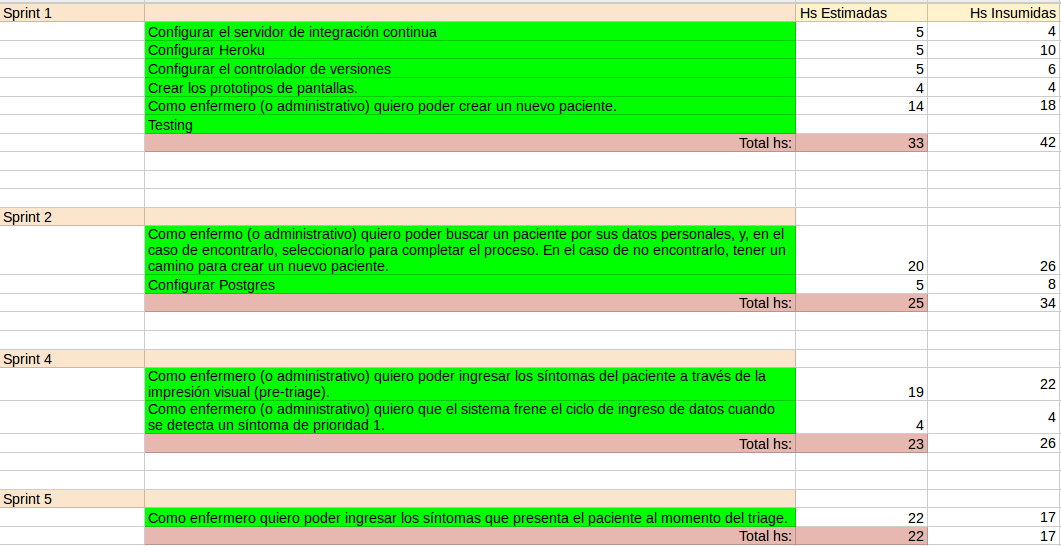
\includegraphics[width=1.2\textwidth]{planificacion.png}}
  \caption{Planificación}
  \label{fig:planificacion}
\end{figure}

A partir de ahí comenzamos con el desarrollo recorriendo las iteraciones planificadas. Al promediar el proyecto hicimos una instalación de prueba en el hospital, y al finalizar el mismo hicimos la instalación definitiva del producto terminado en una máquina de dicha institución.

\subsubsection{Flujo de trabajo en una iteración}
Al inicio de cada iteración estimamos cuanto tiempo nos llevaría cada tarea y enviamos un email con los detalles sobre lo que haríamos durante esa semana. Hacíamos prototipos de las pantallas a realizar que eran validados por el Dr. Reggiani. Dejamos sentado en una hoja de cálculo los detalles de cada tarea: el tiempo de realización estimado, la fecha de realización y el tiempo real insumido (ver figura \ref{fig:tracking}). Luego de cada avance enviamos un reporte por email informando lo realizado y si habían surgido contratiempos. Al finalizar la iteración, enviamos otro email con los detalles de las tareas finalizadas, las que estaban en progreso y las que habían quedado pendientes.

\begin{figure}[h]
  \centerline{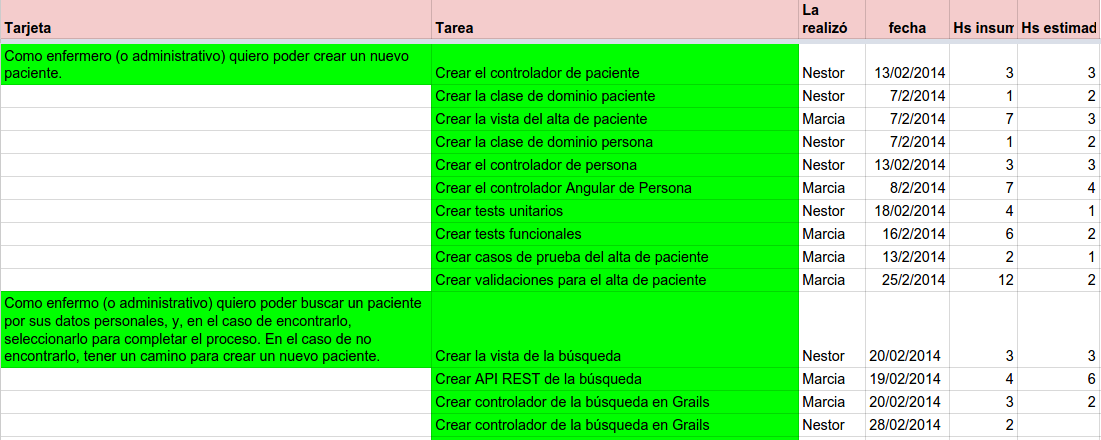
\includegraphics[width=1.2\textwidth]{tracking.png}}
  \caption{\textit{Tracking} de tareas}
  \label{fig:tracking}
\end{figure}

\subsubsection{Herramientas que utilizamos}
Detallamos a continuación las herramientas que utilizamos durante el trabajo.
\begin{itemize}
\item Google Groups\footnote{https://groups.google.com}: comunicación vía email.
\item Google Drive\footnote{https://drive.google.com/}: compartir documentación en línea.
\item Skype\footnote{http://www.skype.com.ar/es/} y Google Hangouts\footnote{https://plus.google.com/hangouts}: comunicación oral de forma remota.
\item Balsamiq\footnote{https://balsamiq.com/}: hacer prototipos de pantallas.
\item Git\footnote{http://git-scm.com/} y Github\footnote{https://github.com/}: versionar y compartir el código (ver sección \ref{cap:repo}).
\item Travis\footnote{https://travis-ci.org/}: servidor de integración continua\footnote{http://es.wikipedia.org/wiki/Integración\_continua}.
\end{itemize}

\subsubsection{Repositorio remoto del código fuente de la aplicación}\label{cap:repo}
El código fuente de la aplicación está disponible en https://github.com/nestor-m/triage

\subsection{Tecnologías}
Todas las tecnologías que utilizamos en el desarrollo de la aplicación son de código abierto. Para desarrollar el \textit{front-end} elegimos AngularJS\footnote{https://angularjs.org/} y para el \textit{back-end} elegimos Grails\footnote{https://grails.org/}.

Cabe aclarar que ambos frameworks cubrieron ampliamente todo lo que nosotros necesitábamos de ellos para hacer este trabajo, por ello sólo utilizamos una pequeña parte de los mismos. Por ejemplo, de Grails casi no utilizamos la parte de las vistas ya que las mismas las desarrollamos del lado del cliente en AngularJS.

Además de estas dos tecnologías utilizamos Bootstrap\footnote{http://getbootstrap.com/} para obtener un diseño amigable para el usuario. Este framework también nos permitió realizar una aplicación \textit{responsive}\footnote{El diseño web adaptable o adaptativo, conocido por las siglas RWD (del inglés, Responsive Web Design) es una filosofía de diseño y desarrollo cuyo objetivo es adaptar la apariencia de las páginas web al dispositivo que se esté utilizando para visualizarla (http://es.wikipedia.org/wiki/Diseño\_web\_adaptable)} que se adapta a cualquier tamaño de pantalla, incluso de teléfonos celulares.

\subsubsection{Sobre la elección de las tecnologías}\label{cap:eleccion_tecnologias}
Como mencionamos anteriormemnte en la sección \ref{cap:itinerario} una de las primeras tareas que realizamos en el proyecto fue la elección de las tecnologías a utilizar. Entre el vasto abanico de posibilidades NodeJS\footnote{http://nodejs.org/} y Grails aparecían como las predilectas ya que son tecnologías modernas y teníamos buenas referencias de ambas. Para decidirnos por una de las dos, desarrollamos un conversor web muy simple de Farenheit a Celcius y en base a los resultados optamos por usar Grails ya que se asemeja más que NodeJS a las tecnologías que veníamos utilizando en las distintas materias a lo largo de la carrera.

Si bien Grails es \textit{full stack}\footnote{Se dice que una tecnología es \textit{full stack} cuando posee todas las herramientas necesarias para desarrollar una aplicación.}, decidimos utilizar una tecnología que resuelva las vistas del lado del cliente, se comunique con el \textit{back-end} mediante una interfaz REST\footnote{La Transferencia de Estado Representacional (Representational State Transfer) o REST es una técnica de arquitectura software para sistemas hipermedia distribuidos como la World Wide Web (http://es.wikipedia.org/wiki/Representational\_State\_Transfer)} 
y sea \textit{responsive}. Así surgió la idea de utilizar AngularJS que cubre ampliamente todos esos requisitos.

Para la elección de la base de datos nos basamos en un tutorial en línea\footnote{https://devcenter.heroku.com/articles/getting-started-with-grails} que recomienda PostgreSQL\footnote{http://www.postgresql.org.es/} como la mejor opción para usar junto a Grails.

\subsubsection{Sobre el \textit{front-end}}
El framework de aplicaciones web AngularJS es desarrollado y mantenido por Google. Es de código abierto y está escrito en JavaScript. La primer versión fue lanzada en el año 2010 y desde ese momento viene ganando espacio en la industria. Este framework es un conjunto de herramientas para la creación de aplicaciones web de una sola página (\textit{single-page applications}). Maneja contenido dinámico y permite extender el vocabulario HTML\footnote{http://es.wikipedia.org/wiki/HTML} obteniendo un entorno más expresivo, legible y práctico para el programador. La filosofía de AngularJS es que la programación declarativa es la que debe utilizarse para generar interfaces de usuario.

\subsubsection{Sobre el \textit{back-end}}
El framework de aplicaciones web Grails es \textit{full stack}, de código abierto y está hecho para la máquina virtual de Java (JVM). Está escrito en Groovy, un lenguaje de programación que a su vez está desarrollado en Java. Uno de sus principios es la convención sobre la configuración que busca decrementar el número de decisiones que un desarrollador necesita tomar, ganando así en simplicidad pero no perdiendo flexibilidad por ello. La primer versión fue lanzada en el año 2006.

Como está desarrollado en Java, Grails es multiplataforma. Además toma de su lenguaje padre tecnologías ampliamente utilizadas en la industria como Hibernate\footnote{http://es.wikipedia.org/wiki/Hibernate}, para la persistencia de datos, y Spring\footnote{http://es.wikipedia.org/wiki/Spring\_Framework}, para la seguridad, la autenticación, las pruebas, la gestión de transacciones, etc.

\subsubsection{Sobre la base de datos}
Para desarrollar una aplicación como la requerida se hizo indispensable utilizar una base de datos para almacenar toda la información ingresada. Los pacientes, los síntomas, las prioridades, los tiempos de espera, etc. son almacenados en una base de datos.

Durante todo el desarrollo de la aplicación utilizamos una base de datos H2\footnote{http://www.h2database.com} que viene embebida en Grails especialmente para utilizar en la etapa de desarrollo. También utilizamos esa tecnología en la instalación de prueba en el hospital. Pero para la instalación definitiva no utilizamos H2 ya que consideramos más apropiado y seguro tener una base de datos independiente del resto del sistema. Por eso utilizamos PostgreSQL\footnote{http://www.postgresql.org.es/} que es un sistema de gestión de bases de datos relacional orientado a objetos.


\subsection{Arquitectura}
Debido a que teníamos que desarrollar una aplicación web capaz de accederse concurrentemente desde varias máquinas al mismo tiempo, decidimos usar una arquitectura cliente-servidor\footnote{http://es.wikipedia.org/wiki/Cliente-servidor} con AngularJS del lado del cliente y Grails del lado del servidor. La comunicación se da mediante peticiones HTTP\footnote{http://es.wikipedia.org/wiki/Hypertext\_Transfer\_Protocol} desde el cliente al servidor y la información viaja en formato JSON\footnote{http://es.wikipedia.org/wiki/JSON}.


\subsubsection{Arquitectura del \textit{front-end}}
El framework AngularJS sigue el patrón de arquitectura Modelo-Vista-Controlador (MVC) de ingeniería de software y alienta la articulación flexible entre la presentación, los datos y los componentes lógicos. Con el uso de la inyección de dependencias, AngularJS lleva servicios tradicionales del lado del servidor, tales como controladores dependientes de la vista, a las aplicaciones web del lado del cliente. En consecuencia, gran parte de la carga en el \textit{backend} se reduce, lo que lleva a aplicaciones web mucho más ligeras.

\subsubsection{Arquitectura del \textit{back-end}}
El framework Grails, al igual que AngularJS, también sigue el patrón de arquitectura MVC. En lo que se refiere a la vista, como en este caso desarrollamos una aplicación de una sola página, entonces tenemos una única pantalla. Por el lado de los controladores tenemos uno por cada clase de dominio. La función principal de los controladores es procesar y responder las peticiones HTTP que llegan desde el lado del cliente. Para hacer esto el controlador se apoya en su clase de dominio (ver figura \ref{fig:diagrama_de_clases}) correspondiente y ésta, a su vez, es la que se encarga de interactuar con la base de datos.

\begin{figure}
\centerline{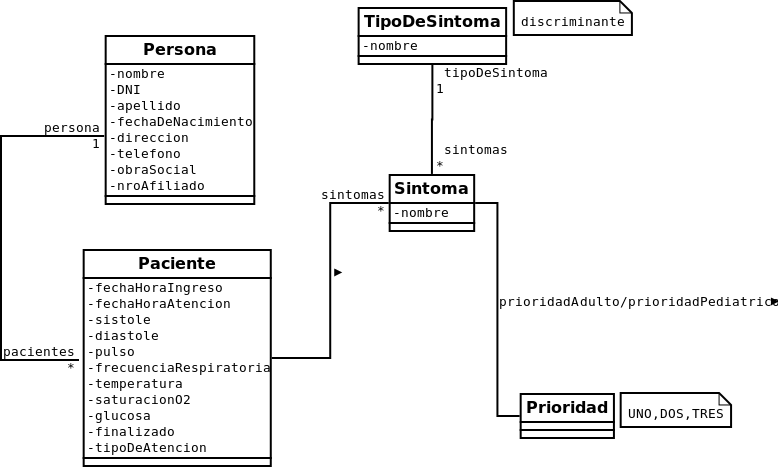
\includegraphics[width=1.2\textwidth]{triage.png}}
\caption{Diagrama de clases del dominio}
\label{fig:diagrama_de_clases}
\end{figure}

\section{Pruebas e instalación}
En esta sección describimos todos los tipos de pruebas que realizamos junto con el desarrollo de la aplicación: pruebas unitarias, de integración y funcionales. En segundo lugar mencionamos algunos problemas con los que nos encontramos al incorporar las pruebas al desarrollo. Por último describimos como realizamos la instalación del producto final.

\subsection{Pruebas}
Desarrollamos la aplicación realizando pruebas unitarias y de integración de cada clase del dominio así como también pruebas funcionales de cada pantalla.

Cada funcionalidad desarrollada tiene su conjunto de pruebas correspondiente. Algunas de las ventajas de usar pruebas automatizadas son las siguientes:

\begin{itemize}
\item Se robustece la aplicación.
\item Se genera confianza en el programador al momento de hacer modificaciones.
\item Se ahorra tiempo.
\item Se disminuye el margen de error en el código.
\end{itemize}

\subsubsection{Pruebas unitarias}
En programación, una prueba unitaria es una forma de comprobar el correcto funcionamiento de un módulo de código. Esto sirve para asegurar que cada uno de los módulos funcione correctamente por separado. Luego, con las Pruebas de Integración, se podrá asegurar el correcto funcionamiento del sistema o subsistema en cuestión. Cabe mencionar que las pruebas unitarias no tienen repercusión en la base de datos. Para realizarlas utilizamos la herramienta nativa de Grails\footnote{\texttt{http://grails.org/doc/latest/guide/testing.html\#unitTesting}} con la biblioteca de Java JUnit\footnote{\texttt{http://junit.org/}}. Así cubrimos el comportamiento de las clases del dominio definidas en el \textit{back-end}

\subsubsection{Pruebas de integración}
Las pruebas de integración son aquellas que se realizan en el ámbito del desarrollo de software una vez que se han aprobado las pruebas unitarias. Se refieren a las pruebas de todos los elementos unitarios que componen un proceso, hechas en conjunto, de una sola vez. Consiste en realizar pruebas para verificar que un gran conjunto de partes de software funciona bien. Las pruebas de integración preceden a las pruebas funcionales del sistema. Cabe mencionar que este tipo de pruebas tiene repercución en la base de datos. Para realizarlas utilizamos la herramienta nativa de Grails\footnote{\texttt{http://grails.org/doc/latest/guide/testing.html\#integrationTesting}}. Con ello cubrimos el comportamiento de los controladores definidos en el \textit{back-end}.

\subsubsection{Pruebas funcionales}
Las pruebas funcionales se basan en la ejecución, revisión y retroalimentación de las funcionalidades previamente diseñadas para el software. Se hacen mediante el diseño de modelos de prueba que buscan evaluar cada una de las opciones con las que cuenta el paquete informático. Dicho de otro modo son pruebas específicas, concretas y exhaustivas para probar y validar que el software hace lo que debe y sobre todo, lo que se ha especificado. Para realizarlas utilizamos CasperJS\footnote{\texttt{http://casperjs.org/}} y Protractor\footnote{\texttt{https://github.com/angular/protractor}} haciendo una simulación del usuario final utilizando la aplicación.

En un primer momento utilizamos CasperJS pero tuvimos muchos problemas para hacerlo funcionar correctamente con AngularJS. Por eso dejamos de usarlo y lo reemplazamos por Protractor.

Para utilizar Protractor necesitamos usar Selenium\footnote{\texttt{http://www.seleniumhq.org/}}, un entorno de pruebas de software para aplicaciones basadas en la web, con un \textit{driver\footnote{\texttt{http://es.wikipedia.org/wiki/Manejador\_de\_dispositivo}}} para el navegador  Chrome\footnote{\texttt{http://www.google.com/intl/es-419/chrome/}}.

\subsubsection{Problemas que tuvimos con el desarrollo de las pruebas}
A continuación detallamos los problemas con los que nos encontramos al utilizar pruebas automatizadas.
\begin{itemize}
\item Hay algunas funciones de Grails que no son soportadas por su ambiente de pruebas. Por eso para que las pruebas pasen, nos vimos obligados a usar solo aquellas funciones que no tenían dicho problema.
\item Tuvimos problemas con Protractor al probar pantallas con ventanas modales. Las ventanas modales son elementos que al aparecer, bloquean la ventana principal de la aplicación. Por eso para poder probar estas pantallas nos vimos obligados a dormir la ejecución de la prueba durante un segundo. Así el modal tenía tiempo para desaparecer y la ventana principal de desbloquearse. Si no hacíamos esto, la prueba fallaba ya que la ejecución de la misma, luego de cerrar el modal, intentaba interactuar con elementos de la ventana principal que aún permanecían bloqueados.
\end{itemize}

\subsection{Instalación}
Acordamos con el Dr. Reggiani hacer la instalación en una máquina del hospital. Como las computadoras están en una misma red entonces la aplicación se encuentra accesible desde cualquier punto del lugar.

La primer instalación (de prueba) la hicimos al promediar el proyecto. El objetivo de la misma fue que los usuarios finales se familiarizacen con el producto, nos dieran \textit{feedback} y propusieran modificaciones de creerlo necesario. La segunda instalación (definitiva) la hicimos al finalizar el proyecto.

Para la instalación de prueba usamos un servidor Tomcat\footnote{\texttt{http://tomcat.apache.org/}} al cual le insertamos el WAR\footnote{\texttt{http://es.wikipedia.org/wiki/WAR\_(archivo)}}(archivo ejecutable que realiza la instalación del producto) de nuestra aplicación que contenía a su vez una base de datos H2\footnote{\texttt{http://www.h2database.com}} embebida.

La instalación final fue similar a la de prueba con la salvedad que no utilizamos la base de datos H2 embebida en Grails. En su lugar instalamos una base de datos PostgreSQL independiente del resto del sistema y, por lo tanto, más segura y confiable.


\subsection{Métricas del proyecto}

\begin{description}
\item[Cantidad de user stories/funcionalidades implementadas] \mbox{} \\
Se implementaron 16 funcionalidades.

\item[Cantidad de iteraciones de trabajo] \mbox{} \\
El proyecto fue realizado en 18 iteraciones de trabajo, cada una de ellas con duración de una semana.

\item[Cantidad de commits en el repositorio] \mbox{} \\
Se realizaron 292 commits en el repositorio de GitHub.

\item[Cantidad de pruebas unitarias] \mbox{} \\
Se realizaron 20 tests unitarios sobre las clases Persona y Paciente.

\item[Cantidad de pruebas de integración] \mbox{} \\
Las pruebas de integración realizadas fueron para las clases de negocio que son tres: los controladores de Persona y Paciente. Son un total de 26 tests.

\item[Cantidad de pruebas funcionales] \mbox{} \\
Se han realizado 14 pruebas funcionales, una para cada funcionalidad de la aplicación. Siempre realizando pequeñas pruebas para cada caso dentro de esa pantalla.


\end{description}

\section{Conclusiones}

\paragraph{}
El presente trabajo abordó el planteo, diseño, implementación, desarrollo y puesta en producción de ``Triage, Sistema de gestión para 
sala de Guardia Hospitalaria''

\paragraph{}
La primer conclusión importante que obtuvimos es la facilidad con la que se pudo desarrollar el trabajo gracias a la interacción continua con el cliente y los directores. Este modo de trabajo permitió llevar el enfoque general del desarrollo hacia el producto final que necesita el cliente. 

\paragraph{}
La segunda conclusión que obtuvimos al terminar el desarrollo de este trabajo es que el contenido en general de la carrera nos dió las herramientas y el conocimiento para poder encarar un proyecto de una magnitud mayor a lo aprendido en cualquiera de las materias cursadas. Permitiendo así la familiarización rápida con tecnologías nunca utilizadas.

\paragraph{}
Finalmente queda por mencionar que, como todo diseño, si bien el trabajo efectuado es de calidad y funcionalidad, queda abierto a mejoras y agregación de nuevas funcionalidades en futuros TIPs.





\newpage 
\begin{thebibliography}{3} 
\bibitem{Derlet} Derlet R, Kinser D, Lou R, et al. Prospective identification and triage of nonemergency patients out of an Emergency Department: a 5 years study. Ann Emerg Med 1996; 25:215-223.
\bibitem{Manual} Manual de procedimiento. Recepción,  Acogida y Clasificación.  MSPBS. Paraguay 2011.
\bibitem{Shore} Shore J, Warden S, The Art of Agile Development, O’Reilly Media, 2007.

\end{thebibliography}

\newpage
\appendix
{\LARGE \textbf{Apéndice}}
\section{Manual de Usuario}
\section{Manual del Usuario}
Las siguientes secciones tienen como objetivo describir y explicar las funcionalidades del Sistema de gestión para sala de Guardia Hospitalaria, que utiliza el método Triage para la recepción de los pacientes. En las mismas, se detalla la funcionalidad de cada pantalla con screenshot y ejemplos básicos y funcionales al manual.

Triage es un método de medicina de emergencias y desastres para la selección y clasificación de los pacientes basándose en las prioridades de atención. La guardia del H.Z.G.A ``Dr.\ Arturo Oñativia'' de la localidad de Rafael Calzada utiliza este sistema para clasificar a sus pacientes. El triage prioriza el compromiso vital inmediato y las posibles complicaciones.
Los pacientes pueden ser clasificados con tres Prioridades:

\begin{description}
\item[Prioridad 1] \mbox{} \\ 
Cuando el paciente tiene posibilidad de sobrevivir y la actuación médica debe ser inmediata.
\item[Prioridad 2] \mbox{} \\ 
Pacientes que presentan una situación de urgencia con riesgo vital.
\item[Prioridad 3] \mbox{} \\ 
Paciente levemente lesionado, que puede caminar y su traslado no precisa medio especial.

\end{description}



\mySection{Ingreso al sistema (\textit{login}) y cambio de contraseña}
En esta sección explicamos como ingresar al sistema y como cambiar la contraseña.

\mySubSection{Ingreso al sistema (\textit{login})}
La primer pantalla que vemos al ingresar a la aplicación es la de \textit{login} (figura \ref{fig:login}).
\begin{figure}[h]
\centerline{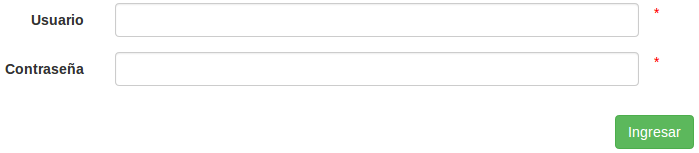
\includegraphics[width=0.7\textwidth]{login.png}}
\caption{Pantalla de ingreso al sistema}
\label{fig:login}
\end{figure}
Allí debemos ingresar correctamente el usuario y la contraseña. Si ingresamos mal alguno de los campos no podremos ingresar al sistema y se nos muestra un mensaje de error (figura \ref{fig:login_fallido}).
\begin{figure}
\centerline{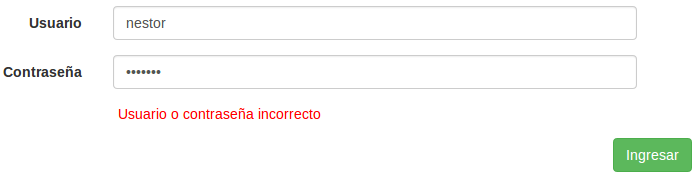
\includegraphics[width=0.7\textwidth]{login_fallido.png}}
\caption{Login fallido}
\label{fig:login_fallido}
\end{figure}

\mySubSection{Cambio de contraseña}\label{cap:cambio_pass}
Para acceder a la pantalla de cambio de contraseña nos dirigimos hacia el nombre del usuario actual y luego a ``Cambiar contraseña'' (ver figura \ref{fig:menu_cambio_pass}).
\begin{figure}
\centerline{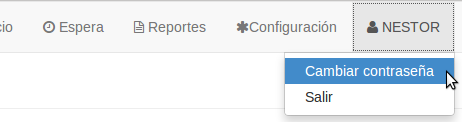
\includegraphics[width=0.7\textwidth]{menu_cambio_pass.png}}
\caption{Menú de cambio de contraseña}
\label{fig:menu_cambio_pass}
\end{figure}
Allí debemos ingresar la contraseña actual y la nueva (dos veces) (figura \ref{fig:cambio_pass}).
\begin{figure}
\centerline{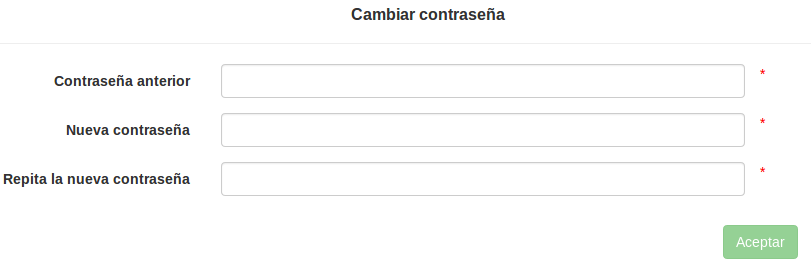
\includegraphics[width=0.7\textwidth]{cambio_pass.png}}
\caption{Cambio de contraseña}
\label{fig:cambio_pass}
\end{figure}
Validaciones a tener en cuenta:

\begin{itemize}
\item El nombre del usuario debe tener al menos tres caracteres.
\item La contraseña debe tener al menos 4 caracteres.
\item Para la contraseña el sistema distingue entre mayúsculas y minúsculas. Si, por ejemplo, nuestra contraseña es ``Clave'' y en la pantalla de \textit{login} ingresamos ``clave'', no podremos ingresar al sistema.
\item Siempre que se crea un usuario nuevo la contraseña por default es ``triage''.
\end{itemize}

\section{Pantalla Inicial}
En esta sección del manual explicaremos cómo ingresar nuevas personas al sistema o cómo buscarlas en el caso de que ya hayan sido atendidas.

\subsection{Ingreso de un nuevo paciente}
En la pantalla de Inicio del sistema (figura \ref{fig:inicio}) 
\begin{figure}
\centerline{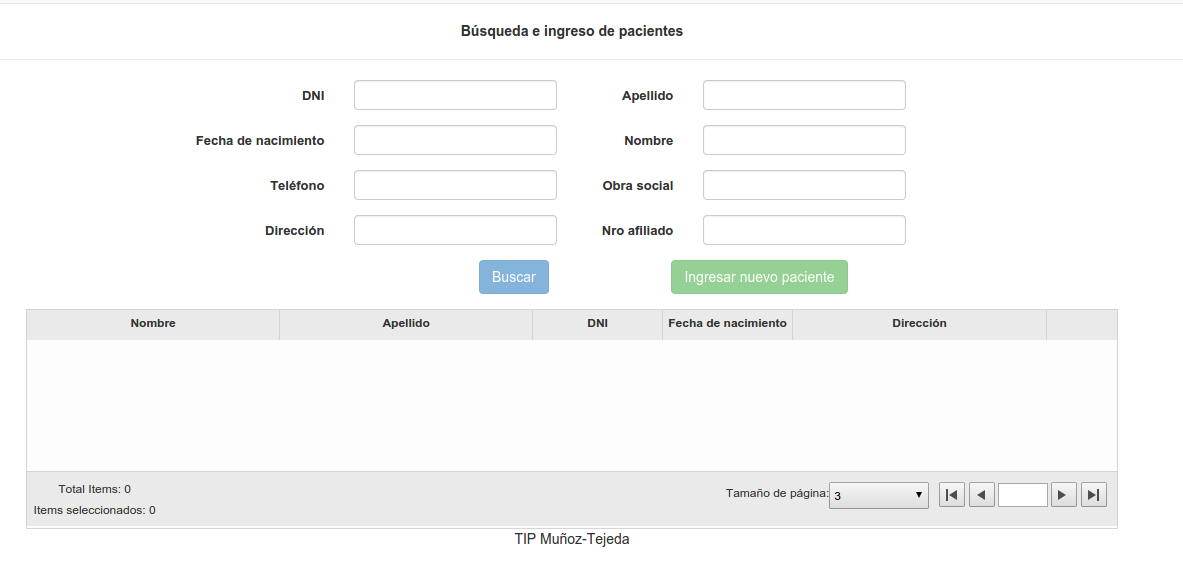
\includegraphics[width=0.99\textwidth]{inicio.png}}
\caption{Pantalla inicial} \label{fig:inicio}
\end{figure}
se pueden ver los campos identitificatorios de las personas. El botón ``Ingresar nuevo paciente'' aparecerá deshabilitado hasta completar los campos obligatorios: DNI, nombre, apellido y fecha de nacimiento (como puede verse en la figura \ref{fig:inicio_nuevo}).
\begin{figure}
\centerline{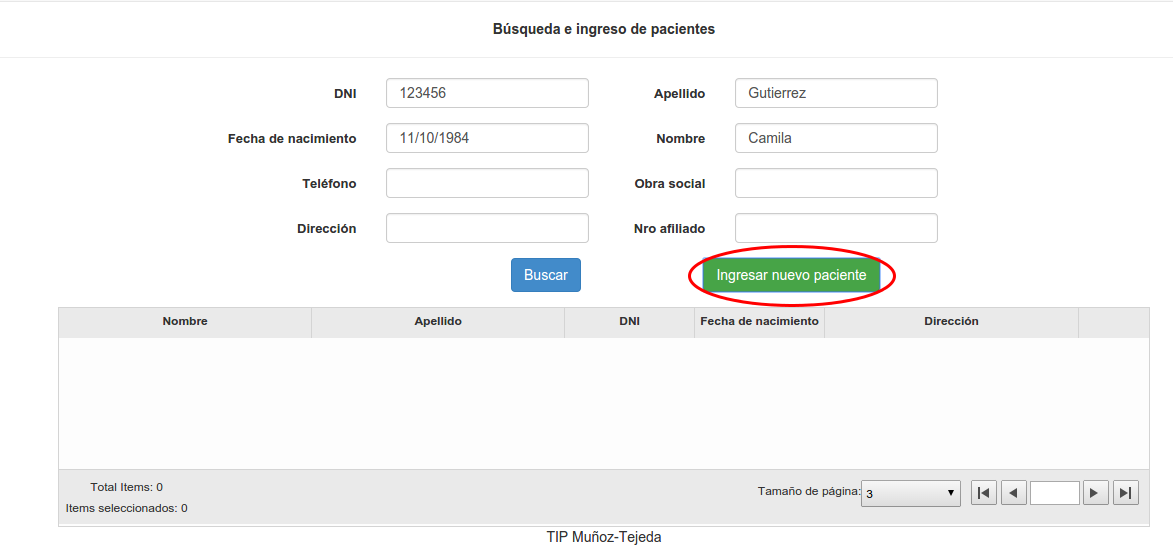
\includegraphics[width=0.99\textwidth]{inicio_nuevo.png}}
\caption{Botón habilitado para poder cargar nuevo paciente} \label{fig:inicio_nuevo}
\end{figure}
Al presionar dicho botón, el sistema guardará los datos de esa persona y redigirá la aplicación a la ventana de Triage para comenzar con la carga de síntomas.

\subsection{Búsqueda e ingreso de un paciente cargado en sistema}
En el caso de que el paciente ya haya recibido atención en la guardia, es posible buscarlo en la aplicación. El botón ``buscar'' apacerá deshabilitado hasta que se complete alguno de los campos (figura \ref{fig:inicio_busqueda}).
\begin{figure}
\centerline{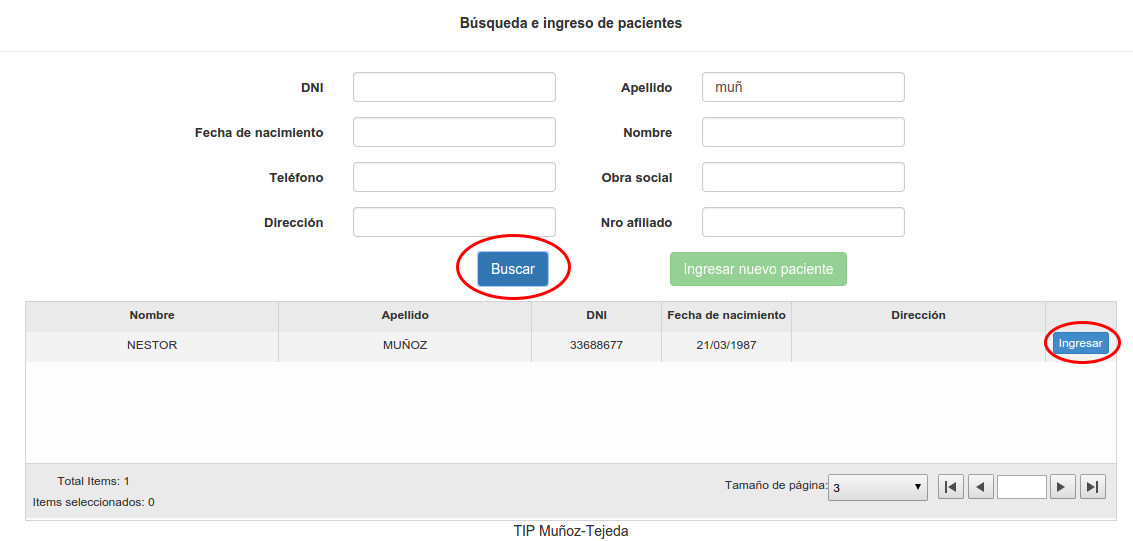
\includegraphics[width=0.99\textwidth]{inicio_busqueda.png}}
\caption{Botón habilitado para poder buscar un paciente y botón para ingresar al paciente a Triage} \label{fig:inicio_busqueda}
\end{figure}
Una vez presionado el botón para buscar, el sistema muestra en el listado inferior la lista de personas que coinciden con los criterios de búsqueda ingresados (ver sección \ref{cap:filtrado_listado}). En el caso de ver a la persona que se está buscando, en la lista aparece el botón ``Ingresar''. Al presionarlo, el sistema redirige la aplicación a la ventana de Triage para comenzar con la carga de síntomas.

\subsection{Filtrado de un listado}\label{cap:filtrado_listado}
Todos los listados de la aplicación pueden ser filtrados para facilitar la búsqueda de algún registro. El modo de filtrado es muy sencillo. Los pasos a seguir son los siguientes:
\begin{enumerate}
\item ingresamos algun texto en el/los campo/s de búsqueda (no hace falta que ingresemos la palabra entera de lo que buscamos, es suficiente si solo ingresamos las primeras letras)
\item presionamos el boton ``Buscar''
\end{enumerate}



\section{Triage}
En esta sección daremos a conocer el camino que recorre la aplicación para cargar los síntomas del paciente.

\subsection{Pantalla inicial de Triage}
La pantalla inicial de Triage (como podemos ver en la figura \ref{fig:triage_inicial}) 
\begin{figure}
\centerline{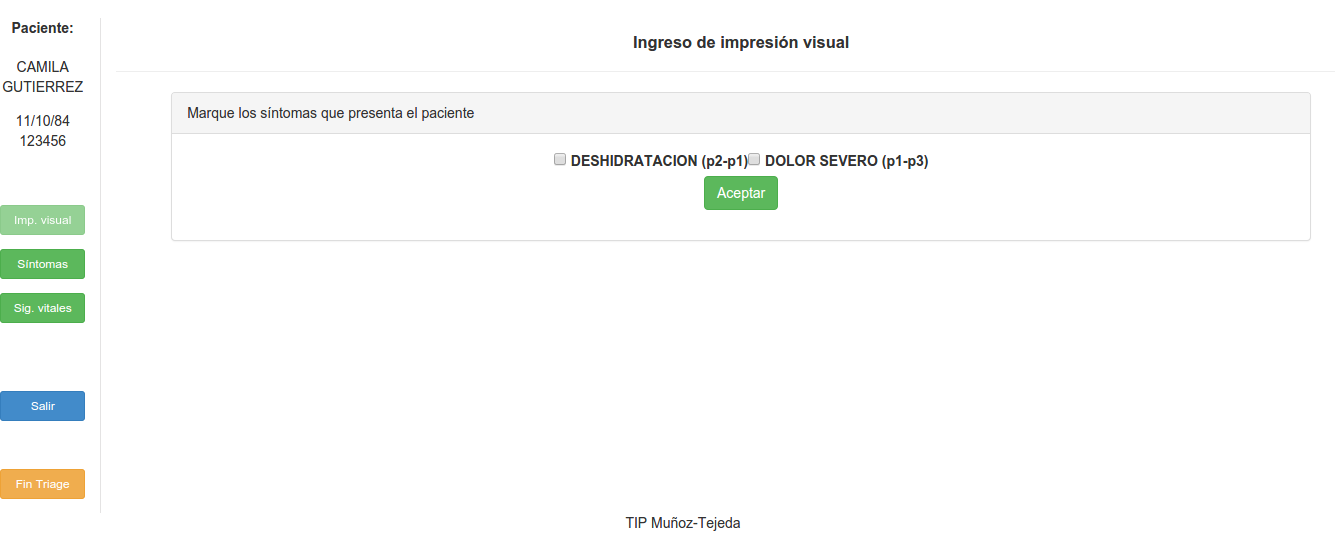
\includegraphics[width=0.99\textwidth]{impresion_visual.png}}
\caption{Pantalla inicial de Triage} \label{fig:triage_inicial}
\end{figure}
tiene una navegación definida por pestañas (que se pueden ver en la parte izquierda de la pantalla). Las pestañas permiten cambiar de pantalla de manera rápida y simple.

\subsection{Impresión Visual}
En la pestaña de impresión visual (figura \ref{fig:triage_inicial}) se cargan los síntomas que el enfermero/administrativo ve en el paciente que está siendo atendido. Una vez seleccionados los síntomas visuales, el usuario debe presionar el botón ``Aceptar''. En el caso de que un síntoma de Prioridad UNO sea seleccionado el sistema corta la interacción con el usuario con un cartel de confirmación (figura \ref{fig:impresion_visual_p1}).
\begin{figure}
\centerline{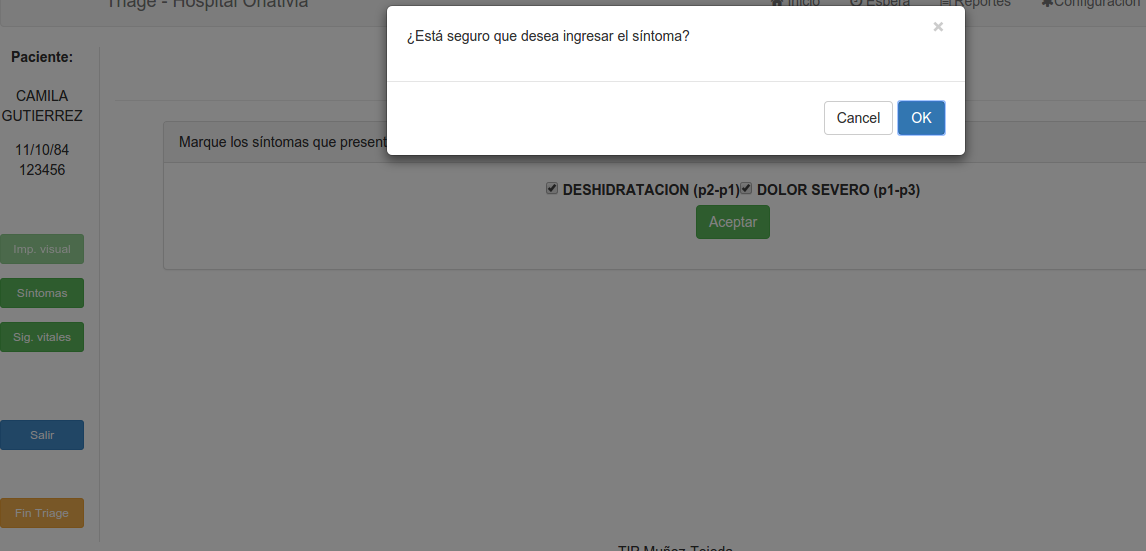
\includegraphics[width=0.99\textwidth]{impresion_visual_p1.png}}
\caption{Pantalla inicial de Triage} \label{fig:impresion_visual_p1}
\end{figure}
Si el usuario confirma, el sistema deriva directamente a la pantalla de Prioridad UNO, mostrando los datos y síntomas del paciente ingresado (figura \ref{fig:prioridad_uno}).
\begin{figure}
\centerline{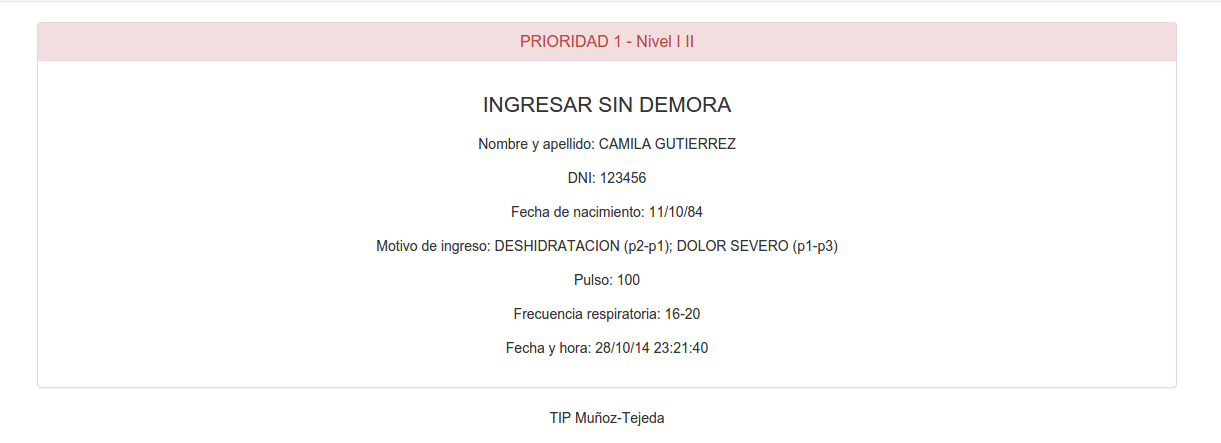
\includegraphics[width=0.99\textwidth]{prioridad_uno.png}}
\caption{Prioridad UNO} \label{fig:prioridad_uno}
\end{figure}

\subsection{Síntomas}
En la pestaña de síntomas (figura \ref{fig:sintomas})
\begin{figure}
\centerline{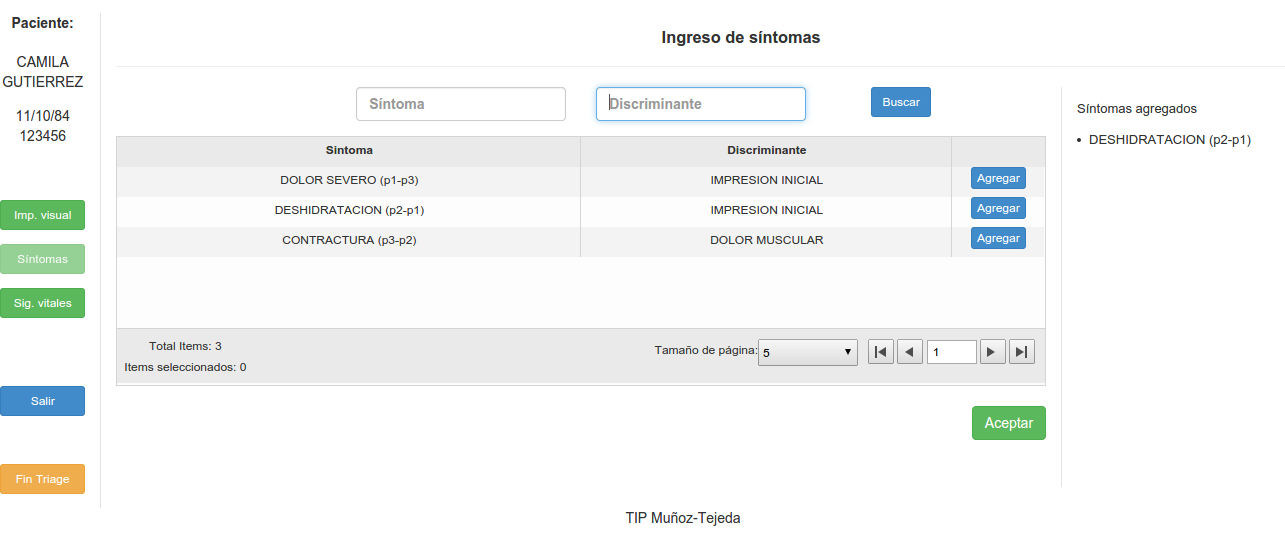
\includegraphics[width=0.99\textwidth]{sintomas.png}}
\caption{Pestaña de síntomas} \label{fig:sintomas}
\end{figure}
van a ser cargados los síntomas que el paciente informe. 

En el cuadro central se pueden ver todos los síntomas cargados en sistema, indicando cuál es su discriminante. Aquí se puede filtrar también por síntoma o discriminante (tal como se explica en la sección 'Filtrado del listado') (Ver figura \ref{fig:sintomas_filtrar}).
\begin{figure}
\centerline{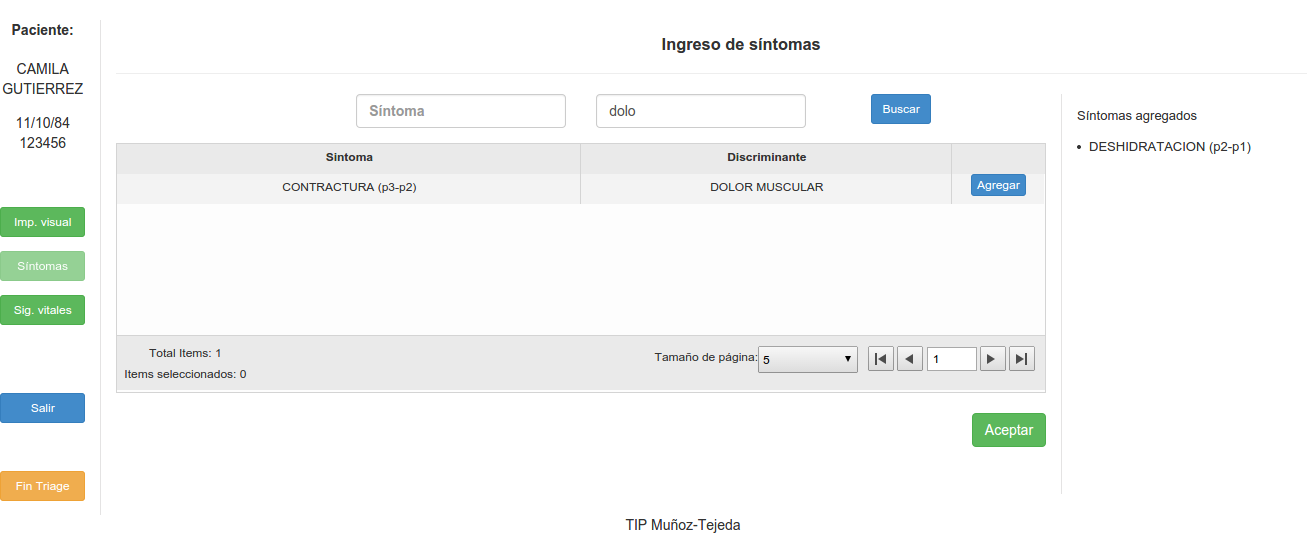
\includegraphics[width=0.99\textwidth]{sintomas_buscar.png}}
\caption{Filtrado en el cuadro de síntomas} \label{fig:sintomas_filtrar}
\end{figure}
Una vez filtrado el listado y encontrado lo que se busca, en cada fila del cuadro se puede ver el botón ``Agregar'' (figura \ref{fig:sintomas_agregar}), que permite cargar un nuevo síntoma al paciente.
\begin{figure}
\centerline{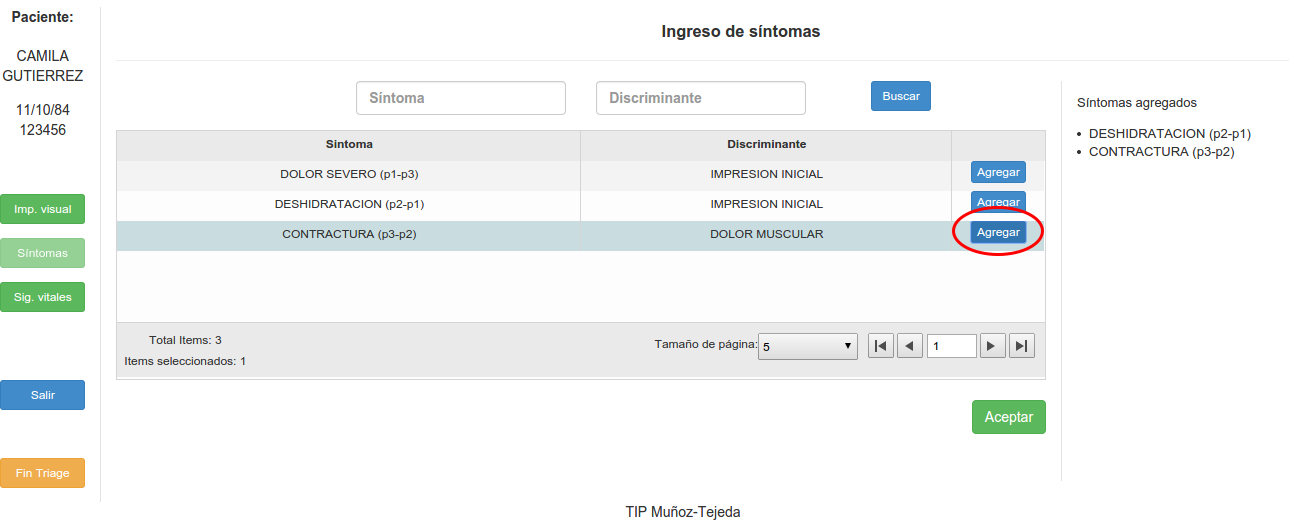
\includegraphics[width=0.99\textwidth]{sintomas_agregar.png}}
\caption{Agregar nuevo síntoma} \label{fig:sintomas_agregar}
\end{figure}
En la parte derecha de la pantalla se pueden ver los síntomas ya cargados. Se puede también eliminar algún síntoma agregado mediante el botón ``Borrar'' (que aparece al pararse con el puntero sobre el elemento a eliminar).

En el caso de ingresar un síntoma con Prioridad UNO,  el sistema corta la interacción con el usuario con un cartel de confirmación. Si el usuario confirma que efectivamente ese es el síntoma a agregar, el sistema deriva directamente a la pantalla de Prioridad UNO, mostrando los datos y síntomas del paciente ingresado (figura \ref{fig:prioridad_uno}).

Al finalizar con la carga, se debe presionar el botón ``Aceptar'' para grabar los síntomas seleccionados.


\subsection{Signos Vitales}
La tercer pestaña del Triage es para completar los signos vitales del paciente (figura \ref{fig:signos_vitales}).
\begin{figure}
\centerline{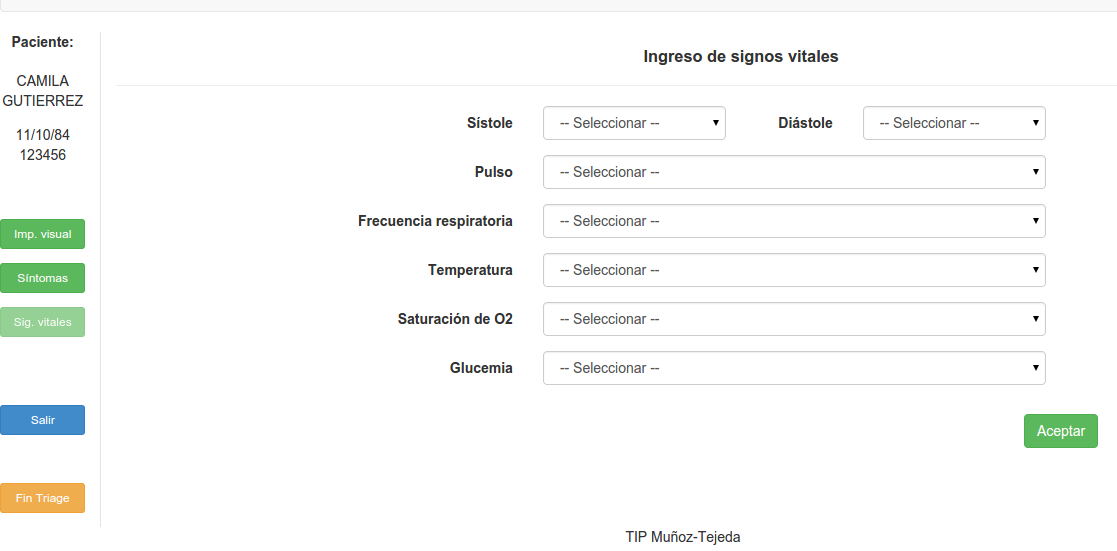
\includegraphics[width=0.99\textwidth]{signos_vitales.png}}
\caption{Signos Vitales} \label{fig:signos_vitales}
\end{figure}
Cada signo vital está definido para ser seleccionado de una lista acotada. En el caso de seleccionar algún valor que corresponda a una Prioridad UNO, el sistema mostrará un mensaje de confirmación. Si el usuario confirma la acción, se corta toda interacción mostrando la pantalla que indica atención inmediata (figura \ref{fig:prioridad_uno}).

Al finalizar de cargar los signos vitales, se debe presionar el botón ``Guardar'' (figura \ref{fig:signos_vitales_guardar})
\begin{figure}
\centerline{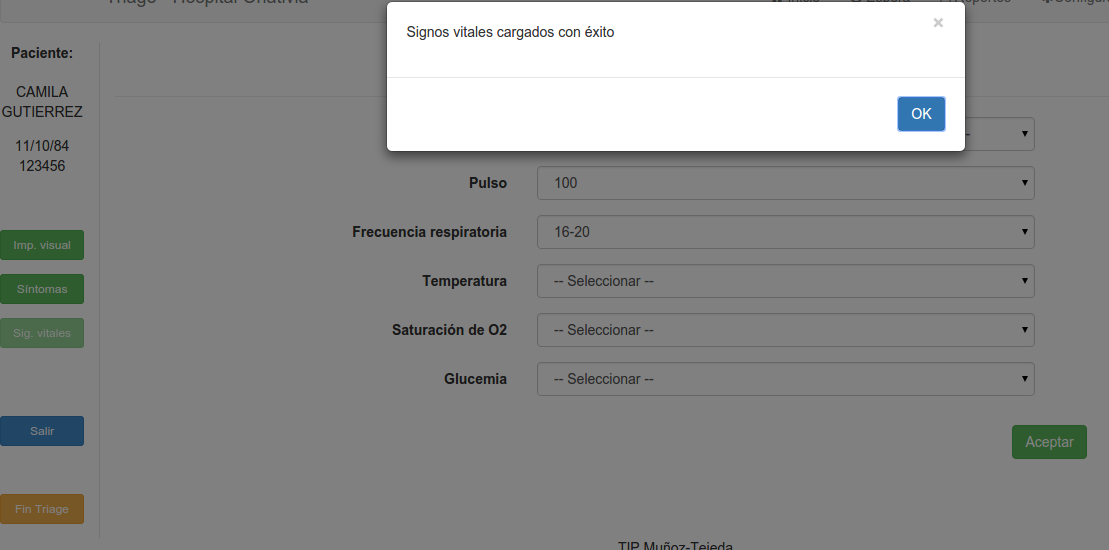
\includegraphics[width=0.99\textwidth]{signos_vitales_guardar.png}}
\caption{Signos Vitales} \label{fig:signos_vitales_guardar}
\end{figure}
y el sistema informará que los datos se han guardado con éxito.


\subsection{Fin de la carga}
Al terminar de cargar los síntomas hay dos caminos:
\begin{description}
\item[Finalizar Triage]  \mbox{} \\
Para finalizar el Triage, se debe presionar el botón sobre la pestaña izquieda llamado ``Fin Triage'' (figura \ref{fig:fin_triage}).
\begin{figure}
\centerline{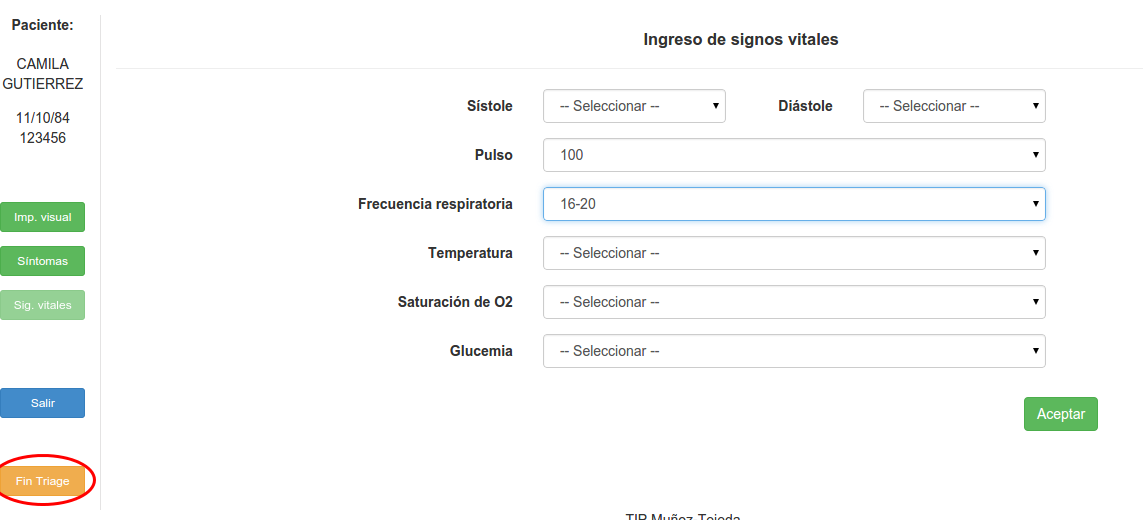
\includegraphics[width=0.99\textwidth]{fin_triage.png}}
\caption{Signos Vitales} \label{fig:fin_triage}
\end{figure}
 Al hacer esto, el sistema calcula la prioridad del paciente, indicando todos los síntomas cargados y sus datos personales. 

Esta acción sólo puede mostrar las pantallas de Prioridad DOS (figura \ref{fig:prioridad_dos}) 
\begin{figure}
\centerline{
\includegraphics[width=0.99\textwidth]{prioridad_dos.png}}
\caption{Prioridad DOS} \label{fig:prioridad_dos}
\end{figure}
y Prioridad TRES (figura \ref{fig:prioridad_tres}), 
\begin{figure}
\centerline{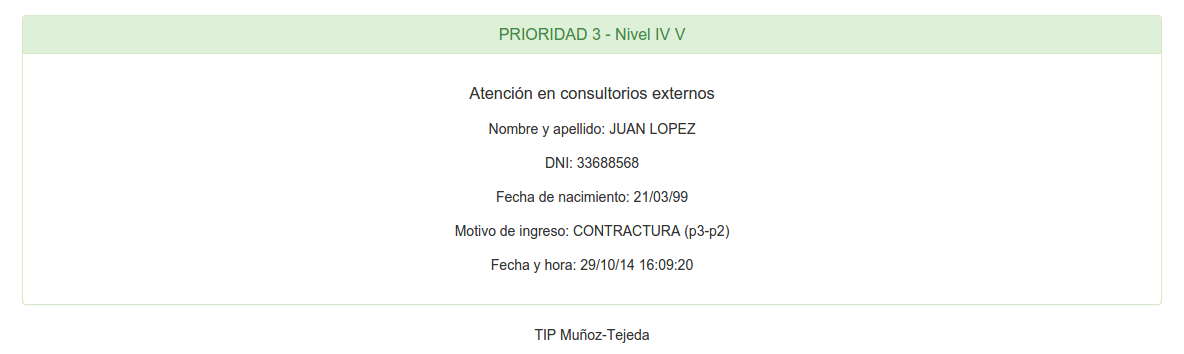
\includegraphics[width=0.99\textwidth]{prioridad_tres.png}}
\caption{Signos Vitales} \label{fig:prioridad_tres}
\end{figure}
ya que la pantalla de Prioridad UNO sólo se presenta al seleccionar un síntoma de Prioridad UNO y corta toda interacción con el usuario.
Finalizar el Triage no quita al paciente de la lista de espera, simplemente calcula su prioridad. 

\item[Salir de la carga]\mbox{} \\
En el caso de querer abandonar la carga de síntomas para poder retomarla más tarde, el sistema provee la acción ``Salir'' (figura \ref{fig:fin}),
\begin{figure}
\centerline{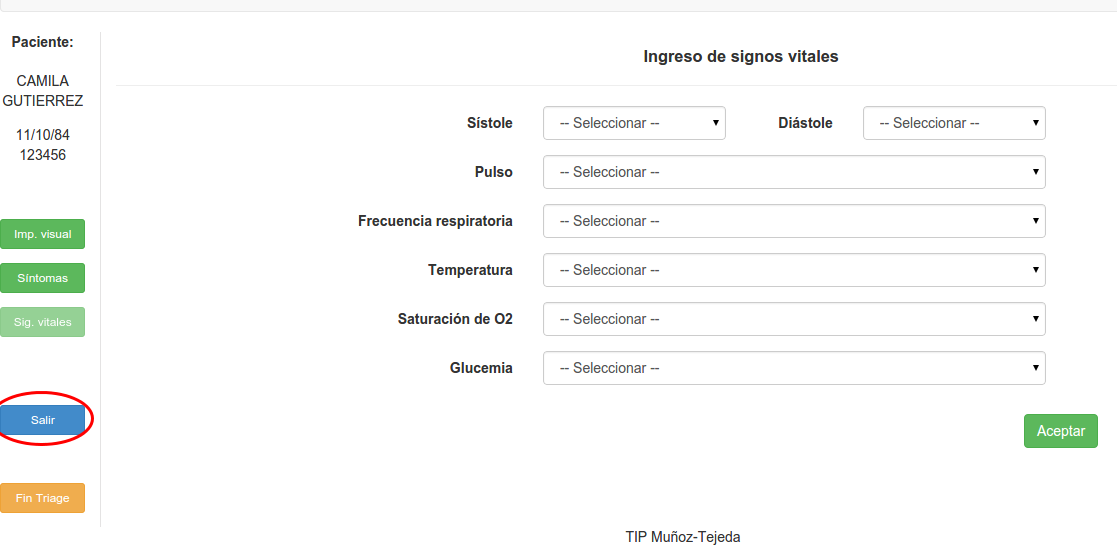
\includegraphics[width=0.99\textwidth]{fin.png}}
\caption{Signos Vitales} \label{fig:fin}
\end{figure}
que permite guardar los síntomas ingresados hasta el momento y poder recuperarlos si se carga el paciente desde la lista de espera.


\end{description}

\section{Pacientes en espera}
En la secciones anteriores se describió la manera de completar el Triage. 

Cada vez que se termina de cargar los síntomas hay dos caminos: ``Fin Triage'' o ``Salir''. Ambas opciones dejan al paciente en una ``Lista de espera'' (figura \ref{fig:espera}).
\begin{figure}
\centerline{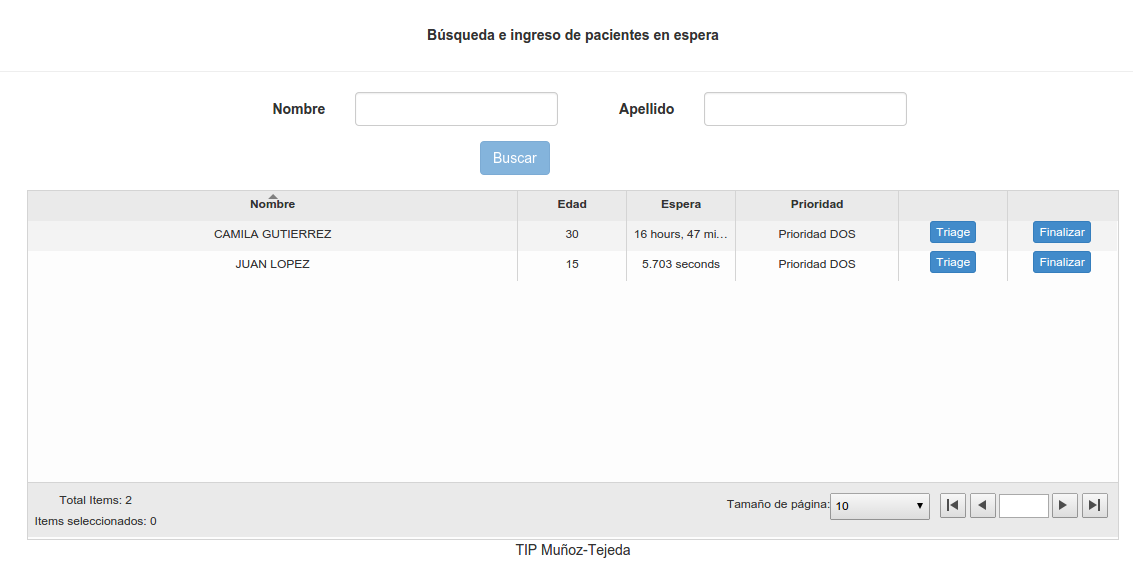
\includegraphics[width=0.99\textwidth]{espera.png}}
\caption{Signos Vitales} \label{fig:espera}
\end{figure}
 La pantalla de lista de espera contiene un cuadro como los vistos anteriormente para la búsqueda de personas así como los filtros para realizar búsquedas en ese cuadro.

Esta pantalla es muy útil cuando la carga de síntomas es realizada por dos personas en ubicaciones físicas distinas. El paciente puede ser atendido en un mostrador (donde se toman sus síntomas, por ejemplo), y luego pasar a un consultorio para la toma de signos vitales. El enfermero en el consultorio debe solamente buscar al paciente en la lista de espera y podrá continuar grabando sus síntomas sin perder ninguna información ya cargada.

\subsubsection{Continuar el Triage}
En el caso de querer continuar el Triage de un paciente en lista de espera, el sistema permite buscar al paciente utilizando el filtro. Una vez localizado, a nivel fila del cuadro encontramos la opción ``Triage'' (figura \ref{fig:espera1})
\begin{figure}
\centerline{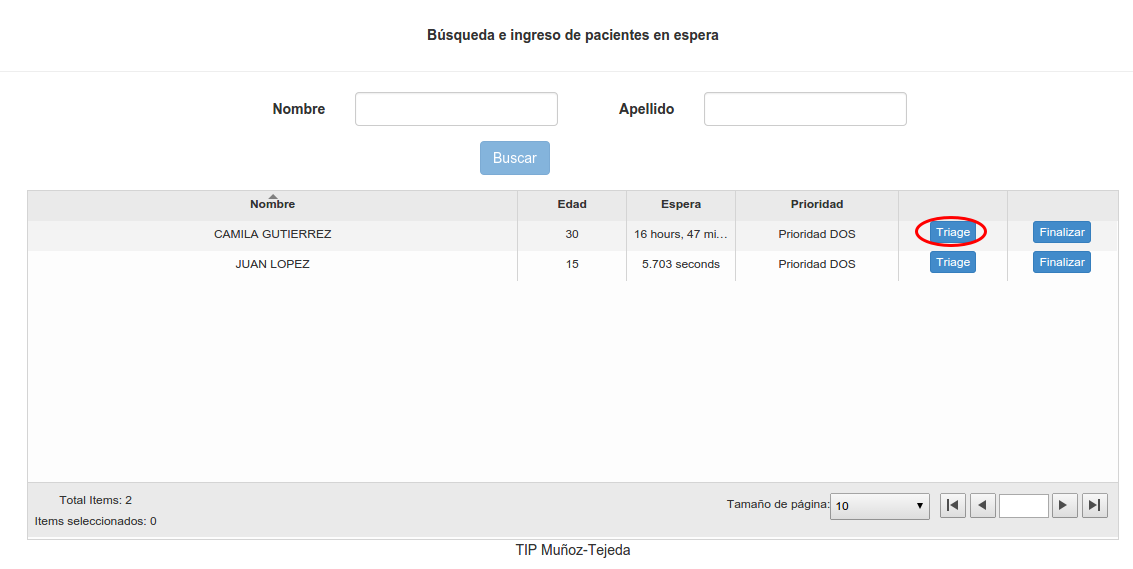
\includegraphics[width=0.99\textwidth]{espera1.png}}
\caption{Signos Vitales} \label{fig:espera1}
\end{figure}
que permite volver a la pantalla de Triage del paciente seleccionado para continuar cargando síntomas.


\mySection{Reportes}
En esta sección explicamos como generar los tres tipos de reportes que realiza el sistema: cantidad de consultas según prioridad, promedio de tiempos de espera según prioridad e historial de atenciones por paciente.

\mySubSection{Reporte de cantidad de consultas según prioridad}
Para acceder a la pantalla del reporte de cantidad de consultas según prioridad nos dirigimos hacia ``Reportes'' y luego a ``Prioridades'' (ver figura \ref{fig:menu_reporte_prioridades}).
\begin{figure}
\centerline{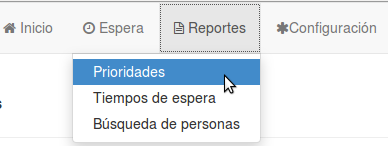
\includegraphics[width=0.7\textwidth]{menu_reporte_prioridades.png}}
\caption{Menú de reporte de prioridades}
\label{fig:menu_reporte_prioridades}
\end{figure}
Allí debemos ingresar la fecha inicial y la fecha final para delimitar las consultas a considerar dentro del reporte. Luego presionamos el botón ``Generar'' para obtener el reporte en pantalla (figura \ref{fig:reporte_prioridades}).
\begin{figure}
\centerline{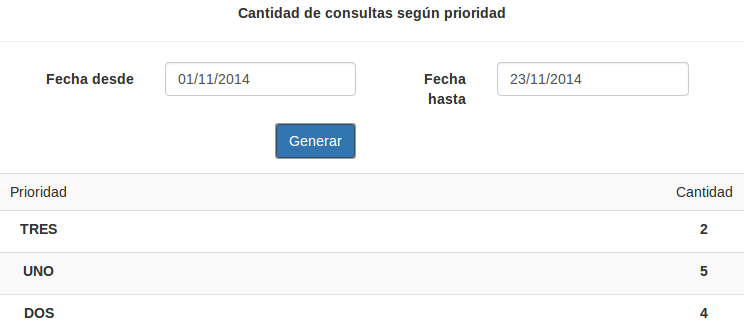
\includegraphics[width=1\textwidth]{reporte_prioridades.png}}
\caption{Reporte de cantidad de consultas según prioridad}
\label{fig:reporte_prioridades}
\end{figure}

\mySubSection{Reporte de promedio de tiempos de espera según prioridad}
Para acceder a la pantalla del reporte de promedio de tiempos de espera según prioridad nos dirigimos hacia ``Reportes'' y luego a ``Tiempos de espera'' (ver figura \ref{fig:menu_reporte_tiempos_espera}).
\begin{figure}
\centerline{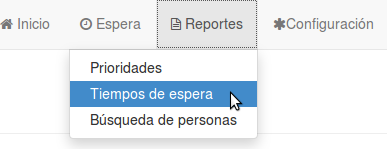
\includegraphics[width=0.7\textwidth]{menu_reporte_tiempos_espera.png}}
\caption{Menú de reporte de tiempos de espera}
\label{fig:menu_reporte_tiempos_espera}
\end{figure}
Allí, al igual que con el reporte de cantidad de consultas, debemos ingresar la fecha inicial y la fecha final para delimitar las atenciones a considerar dentro del reporte. Luego presionamos el botón ``Generar'' para obtener el reporte en pantalla (figura \ref{fig:reporte_tiempos_espera}).
\begin{figure}
\centerline{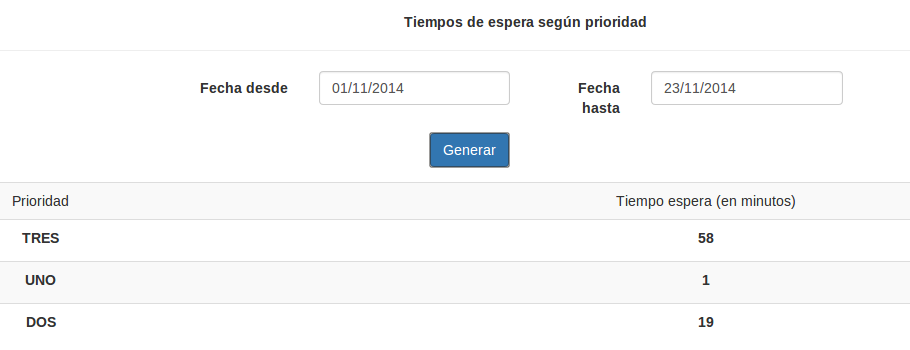
\includegraphics[width=1\textwidth]{reporte_tiempos_espera.png}}
\caption{Reporte de tiempos de espera según prioridad}
\label{fig:reporte_tiempos_espera}
\end{figure}

\mySubSection{Reporte de historial de atenciones por paciente}
Para acceder a la pantalla del reporte de historial de atenciones por paciente nos dirigimos hacia ``Reportes'' y luego a ``Búsqueda de personas'' (ver figura \ref{fig:menu_reporte_pacientes}).
\begin{figure}
\centerline{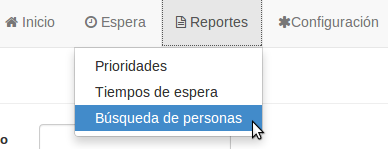
\includegraphics[width=0.7\textwidth]{menu_reporte_pacientes.png}}
\caption{Menú de reporte de historial de atenciones por paciente}
\label{fig:menu_reporte_pacientes}
\end{figure}
Allí podemos buscar el paciente que deseemos por DNI, apellido, fecha de nacimiento o nombre . Una vez encontrado el paciente presionamos el botón ``Detalle'' del listado (ver figura \ref{fig:listado_pacientes}) para ingresar en la pantalla del detalle de atenciones.
\begin{figure}
\centerline{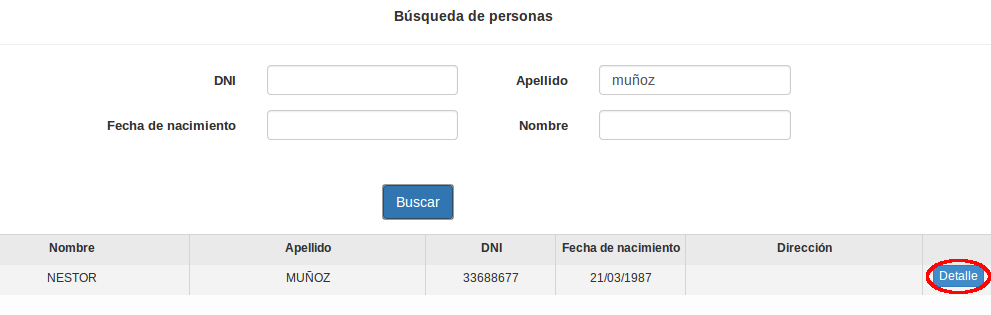
\includegraphics[width=1\textwidth]{listado_pacientes.png}}
\caption{Listado de pacientes}
\label{fig:listado_pacientes}
\end{figure}
Allí se nos muestran los datos personales del paciente más un listado con todas las atenciones que recibió (figura \ref{fig:historial_paciente}).
\begin{figure}
\centerline{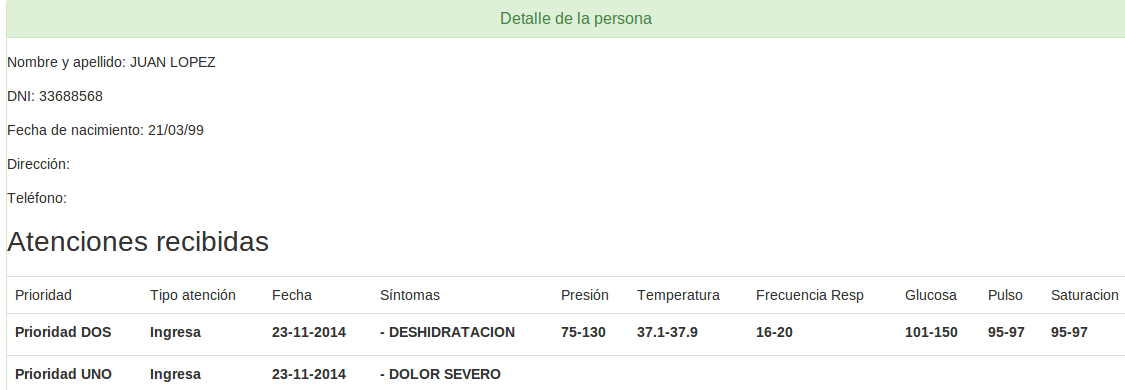
\includegraphics[width=1\textwidth]{historial_paciente.png}}
\caption{Historial de atenciones del paciente}
\label{fig:historial_paciente}
\end{figure}

\mySection{Alta, baja y modificación (ABM) de datos del sistema}
En esta sección explicamos como realizar el alta, baja y modificación de datos del sistema, es decir, síntomas, discriminantes y usuarios.

\mySubSection{Acceso al menú de configuración}
Para acceder al menú de configuración de datos, el usuario actual debe tener el rol de administrador (explicaremos la asignación de roles en la sección \ref{ABM_usuarios}). En caso contrario dicho menú permanecerá oculto (ver figuras \ref{fig:menu_conf_visible} y \ref{fig:menu_conf_oculto}).

\begin{figure}
\centerline{
\includegraphics[width=0.7\textwidth]{menu_configuracion_visible.png}}
\caption{Menú de configuración visible}
\label{fig:menu_conf_visible}
\end{figure}

\begin{figure}
\centerline{
\includegraphics[width=0.7\textwidth]{menu_configuracion_oculto.png}}
\caption{Menú de configuración oculto}
\label{fig:menu_conf_oculto}
\end{figure}

\mySubSection{ABM de síntomas}\label{cap:ABM_sintomas}
Para acceder a la pantalla de administración de síntomas nos dirigimos hacia ``Configuración'' y luego a ``Síntomas'' (ver figura \ref{fig:menu_sintomas}).
\begin{figure}
\centerline{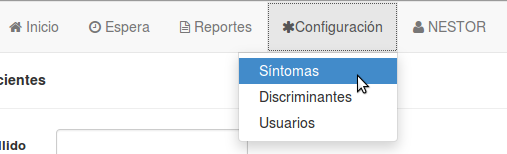
\includegraphics[width=0.7\textwidth]{menu_sintomas.png}}
\caption{Menú de síntomas}
\label{fig:menu_sintomas}
\end{figure}
Allí se nos muestra el listado de todos los síntomas cargados en el sistema (figura \ref{fig:listado_sintomas}).

\begin{figure}
\centerline{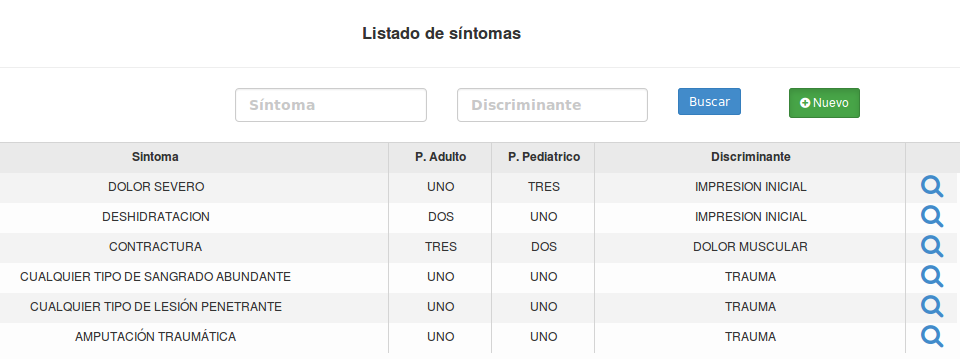
\includegraphics[width=1\textwidth]{listado_sintomas.png}}
\caption{Listado de síntomas}
\label{fig:listado_sintomas}
\end{figure}

\begin{description}
\item[Alta de síntoma] \mbox{} \\
%\subsubsection{Alta de síntoma}\label{cap:alta_sintoma}
En la pantalla del listado de síntomas hacemos click en el botón ``Nuevo'' que nos dirige a la pantalla del detalle del síntoma (figura \ref{fig:detalle_sintoma}).
\begin{figure}
\centerline{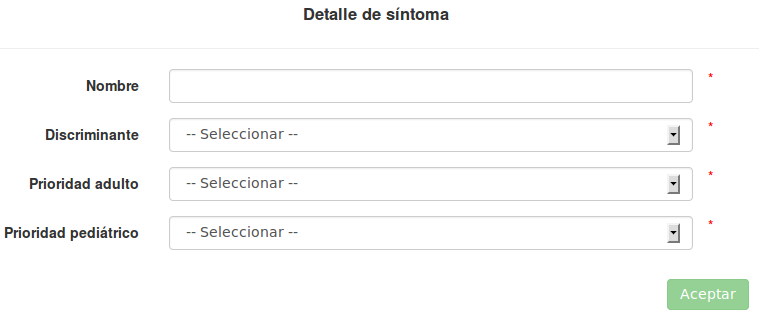
\includegraphics[width=1\textwidth]{detalle_sintoma.png}}
\caption{Detalle de síntoma}
\label{fig:detalle_sintoma}
\end{figure}
Allí debemos ingresar el nombre, el discriminante, la prioridad para adultos y la prioridad para pediátricos. Tener en cuenta que si el discriminante que deseamos no aparece en el listado desplegable entonces primero debemos darle de alta (ver sección \ref{cap:ABM_discriminantes}). Luego de llenar todos los campos, el botón ``Aceptar'' se desbloquea y si le hacemos click debería aparecer un mensaje que confirma que el síntoma fue ingresado con éxito.

\item[Modificación de síntoma] \mbox{} \\
%\subsubsection{Modificación de síntoma}\label{cap:modificacion_sintoma}
Para modificar un síntoma debemos seleccionarlo del listado. Para facilitar la búsqueda del mismo podemos filtrar el listado llenando los campos de ``Síntoma'' y/o ``Discriminante'' (ver sección \ref{cap:filtrado_listado}). Si encontramos el registro buscado hacemos click en el botón ``Ver detalle''(ver figura \ref{fig:sintomas_filtro}) 
\begin{figure}
\centerline{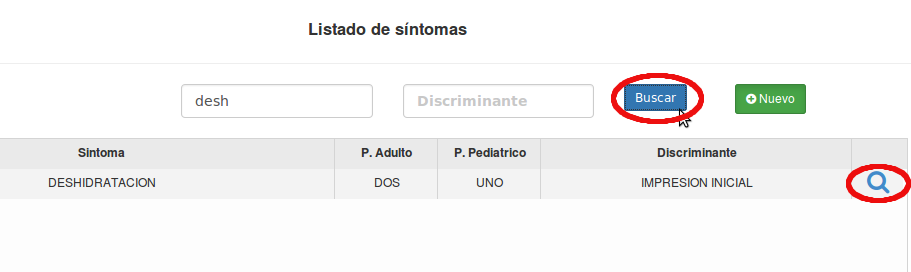
\includegraphics[width=1\textwidth]{sintomas_listado_buscar.png}}
\caption{Listado de síntomas filtrado. Aparecen los botones ``Buscar'' y ``Ver detalle'' señalados en rojo}
\label{fig:sintomas_filtro}
\end{figure}
que nos lleva a la pantalla de ``Detalle de síntoma'' con todos los campos cargados. Allí podemos modificar los valores que deseemos y al presionar el botón ``Aceptar'' debería aparecer el mensaje de confirmación de síntoma actualizado con éxito.

\item[Baja de síntoma] \mbox{} \\
%\subsubsection{Baja de síntoma}
Una vez creados, los síntomas no se pueden eliminar. Solo se pueden modificar como explicamos en la sección anterior. Lo mismo sucede con los discriminantes.

\end{description}

\mySubSection{ABM de discriminantes de síntomas}\label{cap:ABM_discriminantes}
Para acceder a la pantalla de administración de discriminantes nos dirigimos hacia ``Configuración'' y luego a ``Discriminantes'' (ver figura \ref{fig:menu_discriminantes}).
\begin{figure}
\centerline{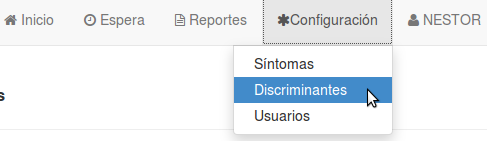
\includegraphics[width=0.7\textwidth]{menu_discriminantes.png}}
\caption{Menú de discriminantes de síntomas}
\label{fig:menu_discriminantes}
\end{figure}
Allí se nos muestra el listado de todos los discriminantes cargados en el sistema (figura \ref{fig:listado_discriminantes}).
\begin{figure}
\centerline{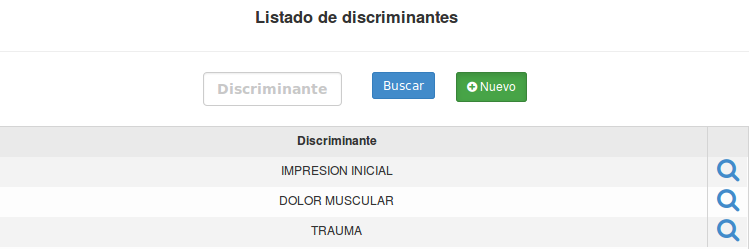
\includegraphics[width=1\textwidth]{listado_discriminantes.png}}
\caption{Listado de discriminantes de síntomas}
\label{fig:listado_discriminantes}
\end{figure}

\begin{description}
\item[Alta de discriminante de síntoma] \mbox{} \\
%\subsubsection{Alta de discriminante de síntoma}\label{cap:alta_discriminante}
En la pantalla del listado de discriminantes hacemos click en el botón ``Nuevo'' que nos dirige a la pantalla del detalle del discriminante (figura \ref{fig:nuevo_discriminante}).
\begin{figure}
\centerline{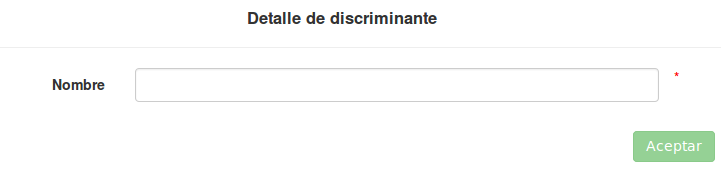
\includegraphics[width=1\textwidth]{nuevo_discriminante.png}}
\caption{Alta de discriminante de síntoma}
\label{fig:nuevo_discriminante}
\end{figure}
Allí debemos ingresar el nombre, lo que desbloquea el botón ``Aceptar'' y si le hacemos click debería aparecer un mensaje que confirma que el discriminante fue ingresado con éxito. Una vez cargado podremos ingresar nuevos síntomas de ese discriminante, como explicamos anteriormente en la sección \ref{cap:ABM_sintomas}.

\item[Modificación de un discriminante de síntoma] \mbox{} \\
%\subsubsection{Modificación de un discriminante de síntoma}
Para modificar el nombre de un discriminante debemos seleccionarlo del listado\footnote{Por cuestiones de lógica del proceso de Triage podemos modificar el nombre de cualquier discriminante a excepción de ``IMPRESIÓN INICIAL''.}. Para facilitar la búsqueda del mismo podemos filtrar el listado llenando el campo ``Discriminante'' (ver sección \ref{cap:filtrado_listado}). Si encontramos el registro buscado hacemos click en el botón ``Ver detalle'' que nos lleva a la pantalla de ``Detalle de discriminante'' con el campo ``Nombre'' cargado y con un listado que nos muestra todos los síntomas de ese discriminante (ver figura \ref{fig:detalle_discriminante}).
\begin{figure}
\centerline{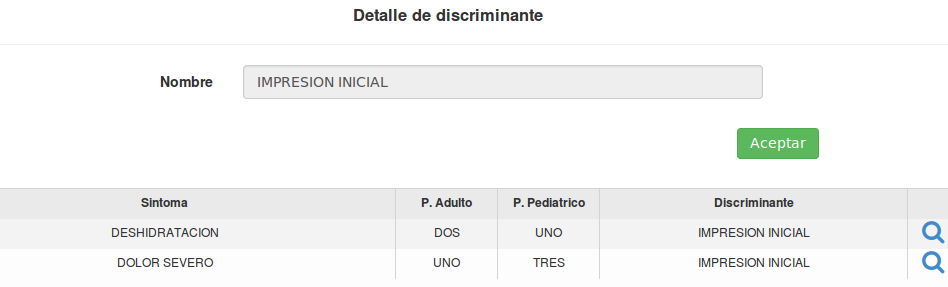
\includegraphics[width=1\textwidth]{listado_sintomas_de_discriminante.png}}
\caption{Detalle del discriminante con listado de síntomas}
\label{fig:detalle_discriminante}
\end{figure}
En esa pantalla podemos modificar el nombre y al presionar el botón ``Aceptar'' debería aparecer el mensaje de confirmación de discriminante actualizado con éxito. También podemos hacer click en el botón ``Ver detalle'' de algún síntoma del listado para ir a la pantalla de ``Detalle de síntoma'' y modificarlo como mostramos anteriormente en la sección \ref{cap:ABM_sintomas}.

\item[Baja de discriminante de síntoma] \mbox{} \\
%\subsubsection{Baja de discriminante de síntoma}
Al igual que los síntomas, una vez creados, los discriminantes no se pueden eliminar. Solo podemos modificarles el nombre como explicamos en la sección anterior.
\end{description}

\mySubSection{ABM de usuarios}\label{ABM_usuarios}
Para acceder a la pantalla de administración de usuarios nos dirigimos hacia ``Configuración'' y luego a ``Usuarios'' (ver figura \ref{fig:menu_usuarios}).
\begin{figure}
\centerline{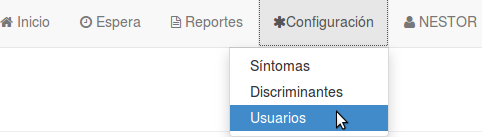
\includegraphics[width=0.7\textwidth]{menu_usuarios.png}}
\caption{Menú de usuarios}
\label{fig:menu_usuarios}
\end{figure}
Allí se nos muestra el listado de todos los usuarios cargados en el sistema (figura \ref{fig:listado_usuarios}).
\begin{figure}
\centerline{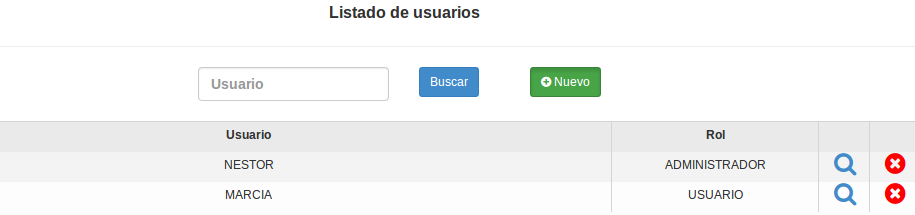
\includegraphics[width=1\textwidth]{listado_usuarios.png}}
\caption{Listado de usuarios}
\label{fig:listado_usuarios}
\end{figure}

\begin{description}
\item[Roles] \mbox{} \\
%\subsubsection{Roles}\label{cap:roles}
Hay dos roles: ``administrador'' y ``usuario''. El usuario con rol ``administrador'' puede ingresar en todas las pantallas de la aplicación. En cambio, el usuario con rol ``usuario'' puede ingresar en todas las pantallas excepto en la de configuración.

\item[Alta de usuario] \mbox{} \\
%\subsubsection{Alta de usuario}\label{cap:alta_usuario}
En la pantalla del listado de usuarios hacemos click en el botón ``Nuevo'' que nos dirige a la pantalla del detalle del usuario (figura \ref{fig:nuevo_usuario}).
\begin{figure}
\centerline{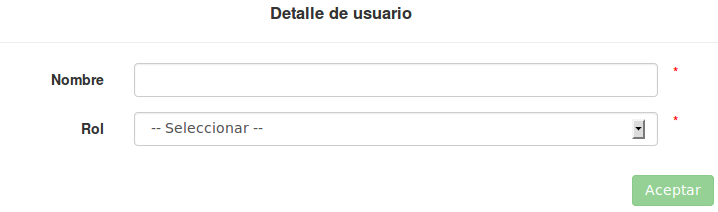
\includegraphics[width=1\textwidth]{nuevo_usuario.png}}
\caption{Alta de usuario}
\label{fig:nuevo_usuario}
\end{figure}
Allí ingresamos el nombre y el rol, y luego presionamos el botón ``Aceptar'' (que desbloqueamos al llenar todos los campos). Nos debería aparecer un mensaje que confirma que el usuario fue ingresado con éxito. Una vez cargado podremos ingresar a la aplicación con ese usuario. Tener en cuenta que todos los usuarios son creados con la contraseña ``triage" (anteriormente explicamos cómo cambiarla en la sección \ref{cap:cambio_pass}).

\item[Modificación de usuario] \mbox{} \\
%\subsubsection{Modificación de un usuario}
Para modificar el nombre o el rol de un usuario debemos seleccionarlo del listado. Para facilitar la búsqueda del mismo podemos filtrar el listado llenando el campo ``Usuario'' (ver sección \ref{cap:filtrado_listado}). Si encontramos el registro buscado hacemos click en el botón ``Ver detalle'' que nos lleva a la pantalla de ``Detalle de usuario'' con todos los campos cargados. Allí podemos modificar los valores que deseemos y al presionar el botón ``Aceptar'' debería aparecer el mensaje de confirmación de usuario actualizado con éxito. Tener en cuenta que el usuario modificado será deslogueado.

\item[Baja de usuario] \mbox{} \\
Para dar de baja un usuario debemos presionar el botón ``Eliminar'' del listado. Si confirmamos la acción deberia aparecer el mensaje de ``Usuario eliminado con éxito'' (figura \ref{fig:eliminar_usuario}).
\begin{figure}
\centerline{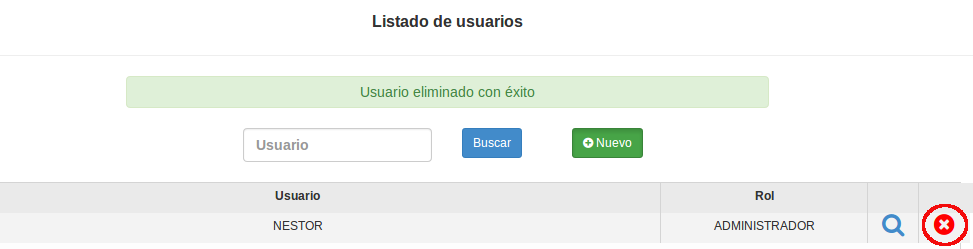
\includegraphics[width=1\textwidth]{eliminar_usuario.png}}
\caption{Baja de usuario}
\label{fig:eliminar_usuario}
\end{figure}
El usuario será deslogueado y ya no podrá ingresar a la aplicación. Tener en cuenta que el sistema no permite que se eliminen todos los usuarios administradores.

\end{description}

\newpage


\end{document}
